\pdfoutput=1
\ifdefined\XeTeXversion\pdfoutput=0 \fi
\documentclass[11pt]{article}
\usepackage[letterpaper, textwidth=5.5in, textheight=9in, centering]{geometry}
\usepackage[T1]{fontenc}
\usepackage{amsmath,amsthm}
\usepackage{newtxtext,newtxmath}
\usepackage{microtype}
\usepackage{graphicx}
\usepackage{booktabs}
\usepackage{array}
\usepackage{longtable}
\usepackage{placeins}
\usepackage[font=small,skip=6pt,tableposition=top]{caption}
\usepackage{xcolor}
\usepackage[numbers,sort&compress]{natbib}
\definecolor{linkblue}{RGB}{0,82,147}
\usepackage[colorlinks=true, linkcolor=linkblue, citecolor=linkblue, urlcolor=linkblue]{hyperref}

\newtheorem{proposition}{Proposition}
\newtheorem{definition}{Definition}

\newcommand{\FO}{\textsc{fo}}
\newcommand{\SO}{\textsc{so}}
\newcommand{\SOp}{\textsc{so}-2/16}
\newcommand{\sg}{\operatorname{sg}}
\newcolumntype{L}[1]{>{\raggedright\arraybackslash}p{#1}}
\newcommand{\Mstar}{\ensuremath{M^{\ast}}}
\newcommand{\lam}{\ensuremath{\lambda^{\ast}}}
\newcommand{\Rcov}{\ensuremath{R_{\mathrm{cov}}}}
\newcommand{\Rcovmem}{\ensuremath{R_{\mathrm{cov,mem}}}}
\newcommand{\LB}{\ensuremath{\mathrm{LB90}}}
\newcommand{\UB}{\ensuremath{\mathrm{UB90}}}
\newcommand{\availurl}{\url{https://github.com/gen4sp/second-order-ttt}}
\makeatletter\@secpenalty=0\makeatother
\setlength{\emergencystretch}{1.5em}

\title{What Second-Order Meta-Gradients Buy in TTT-E2E:\\ Probe Memory at a Language-Modelling Price}
\author{Valentin Lapchevskiy}
\newcommand{\affiliation}{Independent researcher}
\newcommand{\contact}{\href{mailto:v.lapchevskiy@gmail.com}{v.lapchevskiy@gmail.com}}

\makeatletter
\renewcommand{\@maketitle}{%
  \newpage\null\vskip 0.1in
  \hrule height 2pt\vskip 0.22in
  \begin{center}
    {\LARGE\bfseries\linespread{1.15}\selectfont \@title\par}
  \end{center}
  \vskip 0.18in\hrule height 0.6pt\vskip 0.3in
  \begin{center}
    {\large\bfseries \@author\par}\vskip 0.05in
    {\affiliation\par}
    {\small\ttfamily \contact\par}
  \end{center}
  \vskip 0.25in}
\makeatother

\begin{document}
\maketitle

\begin{abstract}
TTT-E2E meta-learns through the gradient steps writing context into its fast weights. Does
second-order (\SO) differentiation through them pay for costing 2.9$\times$ a first-order (\FO) step
in wall-clock time? On a from-scratch text model (25.6M non-embedding parameters) with attention
barriers, a registered equal-GPU-second test finds \FO{} with detached inner gradients and
2.9$\times$ the steps learns a better language model (.43 nats lower adapted loss) but not \SO's
probe memory: its best memory within \SO's loss budget stays .138 [.084, .192] nats below \SO's
(two-sided 80\% interval; retrospective cross-fit), no closer than \FO{} at equal steps. Fresh
seeds replicate this (.139 [.072, .206]); a warmup--stable--decay schedule does not raise its
probe-memory contrast; only partial \SO{} recovers some. \SO's own run was slower than the timing
pilot, so \FO{} received $\approx$92\% of \SO's realised GPU-seconds. No behavioural (passkey)
separation was found. In a toy, attention's copy starves the \FO{} write, blocking recovery; a
linear inner loss, applied at evaluation, rescues \FO{} given a key address. On text this signature
is absent and the mechanism open.
\end{abstract}

\section{Introduction}
\label{sec:intro}

Test-time training (TTT) stores a context in fast weights by gradient steps on a self-supervised loss
\citep{sun2024ttt,behrouz2025titans,zhang2025lact}. TTT-E2E \citep{tandon2025e2e} uses the model's own
next-token loss as that inner loss and meta-trains the whole network through the inner steps.
Differentiating through them is second order (\SO); dropping those terms (first order, \FO) is the
standard cheaper alternative \citep{finn2017maml,nichol2018firstorder}. Here an \SO{} step costs 2.891
\FO{} steps of wall-clock time: with a fixed GPU budget, should one buy \SO{} steps or 2.9 times as
many \FO{} steps?

We registered this question as a test before reading its equal-GPU-second arm, on a from-scratch text model in which
attention barriers leave the fast weights as the only path to distant text (\S\ref{sec:setup}).
Given \SO's GPU-seconds, \FO{} buys language modelling, not \SO's probe memory (\S\ref{sec:text},
Fig.~\ref{fig:frontier}a): with 2.9$\times$ the steps it reaches an adapted loss .43 nats below
\SO's, yet its best probe memory within \SO's loss budget stays .138 nats below \SO's, no closer to
\SO{} than \FO{} at \SO's step count. Fresh seeds replicate this, a
warmup--stable--decay schedule does not raise \FO's probe-memory contrast, and only partial \SO{}
recovers part of the memory. At equal tokens, in a post hoc reading, the memory--loss frontier is two-sided
(Fig.~\ref{fig:frontier}b): \FO{} owns the low-loss end, \SO{} the high-memory end, and an exchange
rate prices the move.

\begin{figure}[t]
  \centering
  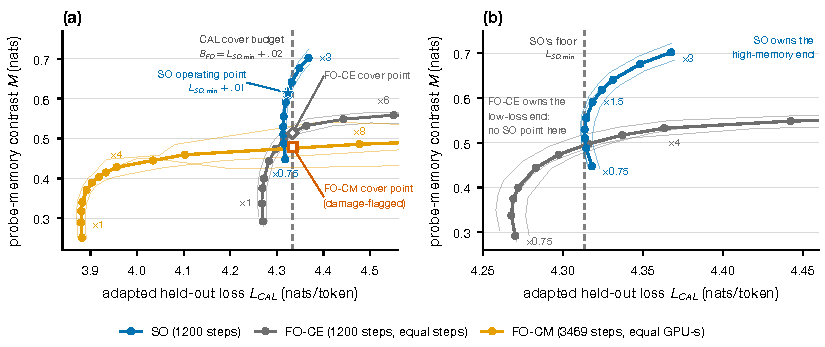
\includegraphics[width=\linewidth]{figs/fig1-frontier.pdf}
  \caption{\textbf{At equal GPU-seconds \FO-CM{} does not reach \SO{}'s probe-memory operating
  point; at equal tokens the frontier is two-sided.} Original study (mini-m, seeds 0--2; the
  replication gives the same labels). (a) Equal GPU-seconds: \SO{}@1200, \FO-CM@3469 and, grey,
  \FO-CE@1200. (b) Equal tokens (post hoc). Bold: seed means over eval-time $\eta$ multipliers; thin:
  seeds. Star: \SO's operating point; open square and diamond: \FO-CM{} (damage-flagged) and \FO-CE{}
  cover points; dashed: budget $B_{\FO}$; $\Rcov$ is the vertical gap from the star. In-sample
  selections; cross-fit changes no label (Appendix~\ref{app:protocol}).}
  \label{fig:frontier}
\end{figure}

Why does \FO{} miss the memory? In a controlled key--value toy (\S\ref{sec:toy}) the cross-entropy
write is proportional to the model's prediction error, so it starves once attention can copy the
value. Contrary to our registered prediction this does not start the loss of a binding; it blocks
recovery. Once keys have an address, a linear inner loss applied at evaluation rescues \FO{} at
\FO{} cost. On text the toy's signature is absent (\S\ref{sec:mechanism}): \FO's deficit grows with distance, not with
predictability at the write, and the text mechanism remains open.

\paragraph{Contributions.}
\begin{itemize}\setlength\itemsep{1pt}
\item A registered, replicated budget test of \SO{} against \FO{} in TTT-E2E on text, read out as a
memory--loss frontier with an exchange rate (\S\ref{sec:text}); one \FO{} rule, one from-scratch model
size and recipe, probe memory only, and no behavioural separation found.
\item A controlled mechanism in which a starved cross-entropy write blocks \FO's recovery, with five
intervention families and an evaluation-carried first-order fix given a key address
(\S\ref{sec:toy}); a cause, not the only one, and what starts the loss is not identified.
\item A negative transfer result: on text the toy's signature is absent, and the text mechanism is
not identified (\S\ref{sec:mechanism}).
\end{itemize}

\section{Setup}
\label{sec:setup}

\paragraph{TTT-E2E and the first-order rule.}
TTT-E2E reads a sequence in chunks and stores what it reads in fast weights. Chunk $c$ is predicted
with fast weights $W_c$, which then take one inner step on the next-token cross-entropy (CE) of that
chunk:
\begin{equation}
  W_{c+1} = W_c - \eta\odot\mathrm{clip}(g_c), \qquad
  g_c = \nabla_W \ell_{\text{inner}}(\text{chunk } c;\, W_c).
  \label{eq:inner}
\end{equation}
Both orders meta-train the slow weights, the initial fast weights $W_0$ and the step sizes $\eta$
through the outer loss of every chunk. \SO{} differentiates through every $g_c$. The \FO{} rule
detaches them, holding the write record fixed, and keeps the direct paths to $W_0$ and $\eta$ and the
same CE inner loss. It is the only \FO{} rule we trained (Appendix~\ref{app:theory} states what it
drops).

\paragraph{Model.}
All text results use one from-scratch model, \emph{mini-m}: 25.6M non-embedding parameters (91.3M in
total), 3.44M of them fast weights in the last two blocks (Table~\ref{tab:hparams}). Sequences are
8192 DCLM tokens \citep{li2024dclm} in chunks of 1024; attention and RoPE reset at chunks 2, 4 and 6,
so after a reset only the fast weights reach earlier text. A step is 16 sequences.

\paragraph{Probe memory.}
A \emph{probe} is the first occurrence, in chunks 4--7, of a 4-gram that also occurs in chunks 0--3,
its \emph{sources}. The probe-memory contrast
\begin{equation}
  M = L_{\text{fP,focal}} - L_{\text{fP,nonfocal}}
  \label{eq:M}
\end{equation}
is how much more the probe loss rises when the inner-loss terms at a probe's sources are removed
(focal) than when a count-matched set of other positions is removed in each chunk (nonfocal).
$\mathrm{fP}_{\text{nonfocal}}=L_{\text{fP,nonfocal}}$ is the absolute probe loss with the source
written.

\paragraph{Frontier, operating point and cover residual.}
Every frontier is an eval-time sweep of one fixed checkpoint over inner step-size multipliers $\eta$.
The adapted loss $L$ (nats/token) is read on 128 held-out documents, split by parity into
\textsc{cal} and \textsc{test}; the no-adapt loss $H_{\text{LM}}$ on 256; $M$ on 1024 others. With
$L_{\text{SO,min}}$ \SO's \textsc{cal} floor over $\eta$, and $\Mstar_a(B)$ the largest $M$ on arm
$a$'s piecewise-linear $\eta$ curve with $L_{\textsc{cal}}\le B$, \SO's operating point is
$L_{\text{SO,min}}+.01$, and an \FO{} arm X is read at the budget $B_{\FO}=L_{\text{SO,min}}+.02$:
\begin{equation}
  \Rcov(\text{X}) = \Mstar_{\SO}(L_{\text{SO,min}}+.01) - \Mstar_{\text{X}}(L_{\text{SO,min}}+.02).
  \label{eq:Rcov}
\end{equation}
With a region of practical equivalence $\text{ROPE}_M=.04$ (registered as $\min(.04,\,.30\,\Delta M(1))$
from the equal-step default-$\eta$ gap $\Delta M(1)=.173$; $\lam\cdot\text{ROPE}_M\approx.007$--.012
nats at the exchange rate of \S\ref{sec:price}), X \emph{does not cover} \SO{} if the lower bound on $\Rcov$ exceeds .04
(\emph{large} if the mean is at least .08), and \emph{covers} only if the upper bounds on both $\Rcov$
and $\Delta_{\text{fn}}$ (X's $\mathrm{fP}_{\text{nonfocal}}$ minus \SO's, at the selected points) are
at most .04; otherwise the test is \emph{underpowered}. The lift
$x=\Mstar_{\FO\text{-CM}}(B_{\FO})-\Mstar_{\FO\text{-CE}}(B_{\FO})$ compares two \FO{} arms at one
budget, so \SO{} cancels. The $\eta$ that maximises $M$ within the budget is selected using $M$, so
the primary analysis cross-fits: $\eta$ is selected on one fixed half of the $M$ documents and $M$
reported on the other, then the halves swap. In-sample selection gives the same labels
(Appendix~\ref{app:protocol}).

\paragraph{Compute match.}
An \SO{} step costs $r=2.891$ \FO{} steps of wall-clock time (RTX 4090; each order at its
fastest-fitting micro-batch, 2 for \SO{} and 4 for \FO; counted FLOPs give 2.02). The
equal-GPU-second arm \FO-CM{} therefore trains $N_{\text{CM}}=1200r=3469$ steps (455M tokens) against
the 1200 (157M) of \SO{} and \FO-CE.
\textbf{Convention:} the budget is \SO's GPU-seconds at its fastest-fitting micro-batch (the
replication's pilot puts the match at $\rho=.997$). \SO{} itself trained at micro-batch 1, which is
slower; against \SO's realised training time the 3469-step arms had $\rho\approx.919$ (original
study) and $\approx.918$ (replication; Appendix~\ref{app:protocol}).

\paragraph{Statistics and status.}
In three-seed text statistics, bounds are one-sided 90\% $t$ bounds over $n=3$ training seeds ($t=1.886$), printed as $[\LB,\UB]$: a \emph{two-sided 80\%
interval}, so the primary rule is one-sided at $\alpha=.10$; secondary labels are not corrected for
multiplicity. Other intervals are labelled where quoted. Results are registered (rule fixed before the
data) unless marked post hoc; our readings are marked ``we read''. The \emph{original study} (seeds
0--2) was registered before any read of its long \FO{} arm, with in-sample selection ($\Rcov=.136$);
its cross-fit values are retrospective. Its operating point and ROPE were fixed after the equal-step
\SO{} and \FO-CE{} frontiers of seeds 0--2 had been read; only \FO-CM{} was unseen. The
\emph{replication} (fresh training seeds 3--5, a denser $\eta$ grid, two schedule arms and a
partial-\SO{} arm) tests the same rule, registered before training, cross-fit included.

\section{At equal GPU-seconds, FO buys language modelling, not SO's probe memory}
\label{sec:text}

\begin{table}[t]
\centering
\caption{\textbf{Every \FO{} arm misses \SO's operating point in both waves.} mini-m, seed means.
\emph{Floor}: adapted \textsc{cal} loss at the $\eta$-grid minimum; $H_{\text{LM}}$: no-adapt loss
(nats/token). \emph{GPU-s}: GPU-seconds relative to \SO@1200 at \SO's fastest-fitting micro-batch ($\rho=.997$);
against \SO's realised micro-batch-1 training the 1.00 arms had $\rho\approx.919$ (original) and .918
(replication). $\Rcov$ (Eq.~\eqref{eq:Rcov}) and $\Delta_{\text{fn}}$ (absolute probe loss with the
source written, minus \SO's), cross-fit (retrospectively in the original study); $[\LB,\UB]$ is a two-sided 80\% interval over three seeds. D:
descriptive; other labels registered. $x$: \FO-CM{} minus \FO-CE; $x_P$: \SOp{} minus \FO-CM.
$^\ddagger$Operating point and ROPE fixed after this arm's frontier
had been read (\S\ref{sec:setup}).}
\label{tab:main}
\footnotesize
\setlength{\tabcolsep}{1.7pt}
\begin{tabular}{@{}lcccll@{}}
\toprule
Arm & Steps (GPU-s) & Floor / $H_{\text{LM}}$ & $\Rcov$ $[\LB,\UB]$ & $\Delta_{\text{fn}}$ $[\LB,\UB]$ & Label \\
\midrule
\multicolumn{6}{@{}l}{\emph{Original study, seeds 0--2}} \\
\SO{}             & 1200 (1.00) & 4.31 / 4.47 & operating point & --- & --- \\
\FO-CE{}          & 1200 (0.35) & 4.27 / 4.37 & .101 [.076, .127] & .168 [.123, .213] & not covered (large)$^\ddagger$ \\
\FO-CM{} (cosine) & 3469 (1.00) & 3.88 / 3.94 & .138 [.084, .192] & .122 [$-.050$, .294] & not covered (large) \\
\quad lift $x$ & & & $-.037$ [$-.072$, $-.002$] & & no closer \\
\midrule
\multicolumn{6}{@{}l}{\emph{Replication, fresh seeds 3--5}} \\
\SO{}             & 1200 (1.00) & 4.31 / 4.46 & operating point & --- & --- \\
\FO-CE{}          & 1200 (0.35) & 4.26 / 4.36 & .061 [.059, .062] & .102 [.085, .120] & not covered (D) \\
\FO-WSD{}         & 1200 (0.35) & 4.19 / 4.28 & .111 [.080, .142] & .168 [.143, .192] & not covered (large; D) \\
\FO-CM{} (cosine) & 3469 (1.00) & 3.88 / 3.94 & .139 [.072, .206] & .163 [.086, .240] & not covered (large) \\
\FO-WSD{}         & 3469 (1.00) & 3.91 / 3.96 & .213 [.175, .252] & .027 [$-.008$, .061] & not covered (large) \\
\SOp{}            & 2793 (1.00) & 3.95 / 4.02 & .067 [.022, .112] & .049 [.003, .095] & underpowered \\
\quad lift $x$ & & & $-.079$ [$-.146$, $-.011$] & & below \FO-CE{} (narrow) \\
\quad lift $x_P$ & & & $+.072$ [$+.023$, $+.121$] & & higher \\
\bottomrule
\end{tabular}
\end{table}

\begin{figure}[t]
  \centering
  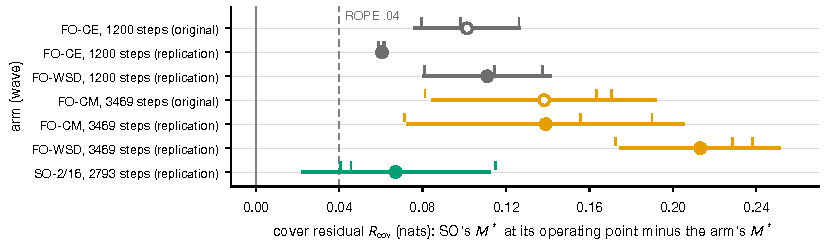
\includegraphics[width=\linewidth]{figs/fig2-rcov.pdf}
  \caption{\textbf{Every \FO{} arm misses \SO's operating point on every seed; only partial \SO{} has
  a cover-residual interval reaching the ROPE boundary.} $\Rcov$ per arm and wave (mini-m),
  cross-fit. Open markers: original study (seeds 0--2); filled: replication (fresh seeds 3--5). Ticks
  are single seeds; the large marker is the three-seed mean and its bar $[\LB,\UB]$, a two-sided 80\%
  interval. Dashed: $\text{ROPE}_M=.04$. Means, bounds and labels: Table~\ref{tab:main}.}
  \label{fig:rcov}
\end{figure}

\subsection{The answer, and its replication}
\label{sec:gpu}

In the original study \FO-CM{} spent its extra steps on the language model: adapted floor 3.88 nats
against \SO's 4.31, no-adapt loss 3.94 against 4.47 (Table~\ref{tab:main}). Probe memory did not follow. \FO-CM's best $M$ within $B_{\FO}$ stays
$\Rcov=.138$ [.084, .192] below \SO's operating point, so the registered label is \emph{not covered,
large}, and \FO-CM{} ends no closer to \SO{} than \FO-CE{} at equal steps ($x=-.037$ [$-.072$,
$-.002$]). The co-condition $\Delta_{\text{fn}}=+.122$ [$-.050$, $+.294$] points the same way but is
not separated from zero, so the label rests on $\Rcov$.

The replication (seeds 3--5, same data) yields the same label, $\Rcov(\FO\text{-CM})=.139$ [.072,
.206], and there \FO-CM's absolute probe-loss gap is separated from zero ($\Delta_{\text{fn}}=+.163$
[$+.086$, $+.240$]). All six seed-level residuals of the two waves lie above the ROPE (.071--.190;
Fig.~\ref{fig:rcov}), and the label holds in every registered sensitivity variant
(Appendix~\ref{app:protocol}).

Two qualifications bound the claim. It is an operating-point statement: \FO-CM's cover points sit at
high $\eta$, where in the original study its focal loss had risen .10--.47 above its own minimum
(the registered damage flag fired on every seed); damage inflates $M$, so the label is conservative
there, but we claim nothing about every $\eta$. And with both arms read at the same floor-relative
budget $L_{\text{SO,min}}+b$, the residual at \SO's own floor ($b=0$) is $\approx.046$, around the
ROPE (descriptive): \SO's edge grows with the budget (\S\ref{sec:price}).

\subsection{Not the schedule, not the step count}
\label{sec:steps}

Is the result an artefact of the cosine schedule stretched to 3469 steps, or of the step count? The
replication tested both with a warmup--stable--decay (WSD) schedule at 1200 and 3469 steps. WSD did
not raise the probe-memory contrast: at 3469 steps its mean residual is descriptively higher than
cosine \FO-CM's ($\Rcov=.213$ [.175, .252]), and at 1200 steps it lies below \FO-CE{}
($\Delta_{\text{shape}}=\Mstar_{\text{WSD-1200}}-\Mstar_{\FO\text{-CE}} =-.050$ [$-.080$, $-.021$];
descriptive). In absolute probe loss with the source written, however, WSD-3469 comes within
$\Delta_{\text{fn}}=.027$ [$-.008$, $.061$] of \SO: its language model predicts many probes without the
source, so part of its lower $M$ is lower headroom (we read this from its probe loss with the source
removed, .17--.21 nats below \SO's per seed at the selected points). \FO-CM's gap persists
(\S\ref{sec:gpu}).

More \FO{} steps moved \FO's probe-memory contrast further from \SO's, not closer. In the replication \FO-CM{} lies
below \FO-CE{} by $x=-.079$ [$-.146$, $-.011$]. The margin is narrow: $\UB=-.011$, seed 4 alone is $-.0095$, and the original study's $x$ supports
only ``no closer''. Under WSD the step effect on $M$ is clearer:
$\Delta_{\text{steps}}=\Mstar_{\text{WSD-3469}}-\Mstar_{\text{WSD-1200}}=-.102$ [$-.114$, $-.090$]
(descriptive). The steps went into language modelling: per seed, $H_{\text{LM}}$ is 3.93--3.97
for both 3469-step arms against 4.36--4.37 for \FO-CE{} and 4.43--4.50 for \SO. We read longer \FO{} training as extending the frontier's low-loss end (\S\ref{sec:price}),
not its high-memory end.

\subsection{What recovers memory}
\label{sec:recover}

Only one arm moved toward \SO. \SOp{} applies second-order meta-gradients to 2 of the 16 sequences of
every batch and first order to the rest, and trains 2793 steps at its own pilot-timed
equal-GPU-second horizon. It lies above \FO-CM{} ($x_P=+.072$ [$+.023$, $+.121$]), but its cover of
\SO{} is underpowered: $\Rcov=.067$ [.022, .112], and every seed residual (.115, .046, .041) exceeds
the ROPE. Descriptively, \SOp{} recovers $\approx52\%$ of \SO's probe-memory edge over \FO-CM{}
(.072/.139) while keeping $\approx83\%$ of \FO-CM's no-adapt language-model gain over \SO, on all three
seeds. The two shares combine different measures (no-adapt $H_{\text{LM}}$ and the selected adapted
$M$), so this is a trade-off point, not a joint optimum, and only one row fraction was tested. At
equal steps no cheaper lever we tried closes \SO's default-$\eta$ memory gap
(Appendix~\ref{app:protocol}, Table~\ref{tab:knobs}), whereas in the toy partial and late \SO{} (cf.\
derivative-order annealing \citep{antoniou2019maml}) each restore retention in 12/12 seeds
(Appendix~\ref{app:toy}).

\subsection{The price: a two-sided frontier and an exchange rate}
\label{sec:price}

With tokens rather than GPU-seconds held equal (\SO{} and \FO-CE, both 1200 steps), the frontier is
two-sided (Fig.~\ref{fig:frontier}b; a post hoc reading of registered reads). \FO-CE{} owns the
low-loss end: its adapted floor is .034--.053 nats below \SO's per seed and its $H_{\text{LM}}$ .096
lower. \SO{} owns the high-memory end: at \SO's floor $+.01$ its $M$ exceeds \FO-CE's at equal $L$ by
$+.108$ (lower bound $+.080$), and the replication's equal-step residual is $\Rcov(\FO\text{-CE})=.061$
[.059, .062]. At \SO's own floor the edge is $\approx+.02$, so neither order dominates; two post hoc
controls argue against inflated $\eta$ as the source of \SO's edge (Appendix~\ref{app:protocol}).

The exchange rate $\lam$ is the first $w\in[0,2]$ at which \SO's best $L-wM$ equals \FO's, over
interpolated points with $L\le L_{\text{SO,min}}+.05$, in nats of per-token loss per nat of per-probe
memory. Against equal-step \FO-CE, $\lam=.16$--$.30$ in the original study and .24--.44 in the
replication; against equal-GPU-second \FO-CM, 1.35--1.74 and 1.46--1.77 (per seed; the replication's
values are estimates, none censored by the window). $\lam$ depends on the grid and window and is
not portable across probes, sizes or corpora. Cross-segment repeats, the targets only fast
weights can serve, are 1.61\% of DCLM targets, so a nat of per-probe $M$ worth a nat on each such
target gives $w_{\text{tok}}\approx.016$, ten times below every $\lam$ estimate; we read this as
favouring \FO's points at both budgets on these curves.

\section{Why FO loses memory: a starved write in a controlled toy}
\label{sec:toy}

The text result says what \SO{} buys, not why \FO{} misses it; a toy isolates one reason.

\subsection{The echo task and its two barriers}
\label{sec:twobarriers}

Each echo sequence writes 16 key--value pairs in its first chunk, as events \texttt{W v k v}: a write
marker, the value, the key and the value again; 300 tokens later a query \texttt{Q k} must
return $v$, beyond the 253-token reach of its sliding-window attention, so only a
fast-weight head can answer; each sequence draws a fresh map, so no in-weights solution exists. The
model is a small transformer with a fast MLP head on top, meta-trained as in
\S\ref{sec:setup} for 1500 outer steps; \emph{retention} is query accuracy $\ge0.90$ at step 1500
(chance 1/16; Appendix~\ref{app:hparams}).

The task has two barriers. Without a key code, plain \FO{} never binds: \SO{} acquired the binding in
7/10 and 7/12 seeds against 0/10 and 0/12 for \FO, and key addressability was at chance (1/16) in all
14 probed models that ended unbound, an address barrier rather than a starved write. A frozen random key code
added to the fast head's input (\emph{$+$emb}) removes it and exposes the second barrier: at fixed
inner step sizes \FO-CE{} acquired the binding in 16 runs and retained it in none, while \SO{} acquired
15 and retained 15/15; a registered fresh-seed replication at $\eta=40$ gave \FO-CE{} 0/15 against
\SO{} 12/12 (Appendix~\ref{app:toy}, Table~\ref{tab:twobarriers}).

\subsection{One write, followed through}
\label{sec:starved}

Take the event \texttt{W 7 k 7}, which binds key $k$ to value 7. At the key token (a \emph{kv}
position, whose next-token target is the written value) the target is the second 7, and attention
can copy it from the 7 just before the key. After the chunk is read, the CE
inner update associates the representation of $k$ with 7, with a strength proportional to the
prediction residual $1-p(7)$ at that position; the query \texttt{Q k}, 300 tokens later, can be
answered only from the fast weights. Early in training the copy is
poor and the residual gives a useful write; once the copy is reliable, the residual and the write
shrink together. Under \FO{} nothing in the outer gradient keeps the write up; under \SO{} the outer
loss at the query can. This is an inner-loop analogue of gradient starvation
\citep{pezeshki2021gradient}: a pathway that already predicts the target suppresses the gradient
another pathway needs. We call it \emph{write starvation}.

\subsection{Starvation blocks recovery; it does not start the loss}
\label{sec:chron}

We registered the prediction that starvation starts the loss, with the residual persistently low at
and before the binding is lost. It was \emph{falsified} (0/6 seeds): the residual at the loss was
still .14--.63 (.21--.68 in 15 fresh seeds). The dense logs show something else (Fig.~\ref{fig:chr};
alignment post hoc, reading registered and replicated on fresh seeds): every main arm loses the
binding at first, and the arms differ in whether it returns. \SO{} recovers
within 10--30 steps (11/11) and an arm with 3\% copy noise in 12/12, while \FO-CE{} recovers in 0/15
and its residual collapses by two more decades, to $3\times10^{-4}$--$1.6\times10^{-3}$.

Starvation, once established, therefore \emph{blocks recovery}. A residual floor switched on after the
collapse, in a run forked from the starved state, restores the binding in 12/12 fresh seeds against
1/12 for an unmodified fork ($p=0.00049$). At that dose (.03) the floor is needed in training (the
unmodified fork's weights read with it re-acquire in 1/12) and at evaluation (the recovered models read with plain CE: 0/12 bound); at .10
and above it acts partly through the read.
Masking the outer CE at the write positions from acquisition on prevents a sustained loss in 14/15
\FO{} seeds (count-matched control 0/15), but this identifies neither the trigger nor a mediator. We
read the starved write as \emph{a} cause of \FO's failure to recover, not the only one; what triggers
the loss is not identified (Appendix~\ref{app:toy}).

\begin{figure}[t]
  \centering
  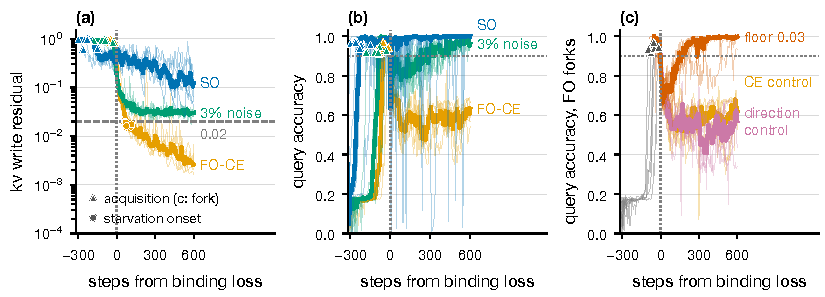
\includegraphics[width=\linewidth]{figs/chr-chronology.pdf}
  \caption{\textbf{Every arm loses the binding at first; only \FO-CE's kv residual then collapses,
  and only \FO-CE{} never recovers.} Echo, fixed $\eta=40$, aligned at each seed's binding loss
  (dotted). Triangles: acquisition (in (c), the fork); dots: registered starvation onset (two
  consecutive logs with residual below 0.02), reached only by \FO-CE. (a) Median kv write residual
  (dashed: 0.02). (b) Query accuracy, 6 seeds per arm. (c) Runs forked from an \FO{} seed's main run
  at acquisition: unmodified CE, kv residual floored at 0.03, same-norm direction control; grey: main
  run before the fork. Thin: seeds; thick: medians over $\ge3$ seeds. Events registered; alignment and recovery reading post hoc.}
  \label{fig:chr}
\end{figure}

\subsection{Interventions that restore the write restore retention}
\label{sec:interv}

Five intervention families that restore the write, or remove the copy that starves it, restore \FO{}
retention; same-count site controls, where tested, do not
(Table~\ref{tab:interventions}). This supports the prediction-coupled write as a cause, not the only
one: every intervention changes more than the residual, and the registered outer-mask mediator fell short
(6/10; 8/10 required).

\begin{table}[t]
\centering
\caption{\textbf{Interventions that restore the write, or remove the copy that starves it, restore
\FO{} retention; same-count site controls do not.} Echo, \FO-CE$+$emb, paired seeds; the unmodified
anchor retained 0/10 each time; $\bar z$: mean logit. $^\dagger$Apple MPS; replicated on CUDA (10/10 against 0/10). Full table with exact tests:
Appendix~\ref{app:toy}, Table~\ref{tab:interventions-full}.}
\label{tab:interventions}
\small
\setlength{\tabcolsep}{4pt}
\begin{tabular}{@{}llcl@{}}
\toprule
Intervention & What changes & Retained & Control (retained) \\
\midrule
Outer-loss mask at kv$^\dagger$ & no direct outer CE at kv & 10/10 & adjacent targets: 0/10 \\
Copy-edge attention mask & kv cannot attend to its source & 10/10 & --- \\
Linear inner loss at kv & inner loss at kv is $\bar z-z_y$ & 10/10 & next position: 0/10 \\
Copy noise, $q\in\{3,5,10\}\%$ & copy wrong w.p.\ $q$ & 18/18 & $q=1\%$: 0/6; filler: 0/6 \\
Separate kv step size & own $\eta$ at kv & 8/10, 10/10 & --- \\
\bottomrule
\end{tabular}
\end{table}

\subsection{The write target, a first-order fix given an address, and two other domains}
\label{sec:toyfix}

At matched update norm the \emph{write target} matters: replacing CE by the prediction-independent
linear loss (mean logit minus target logit) at every position closes the echo deficit
(difference-in-differences $+.454$ [$+.294$, $+.615$], a two-sided 90\% $t$ interval over six
seeds). Given a
frozen key address, the linear inner loss removes \FO's retention failure at first-order cost (10/10
at kv only, 10/10 everywhere, 12/12 on fresh seeds). The rescue is carried by evaluation: on fresh
seeds, CE-trained models read with the linear loss bind in 12/12 and linear-trained models read with
CE in 0/12. It has a price. Without the key code it
never binds (0/12; an address-keeping auxiliary loss restores 12/12, a filler control 0/12); on re-assignment it mostly keeps the old map (new-map accuracy .30--.48, where \SO{} reaches
.92--.93; descriptive); and switched onto CE-trained 125M weights at test time it cost .85--1.4 nats,
so it is not a drop-in text fix. On an in-context Markov task the linear loss beats \FO-CE{} by .026
nats and, on the last quarter of positions, \SO-CE{} by .005, so \FO{} does not fail at memory in
general. A toy \SO{} step costs about one \FO{} step, so the toy says nothing about compute.

\paragraph{A symbolic world model.}
In a symbolic world-model stream (SCM; Appendix~\ref{app:domains}), no fixed \FO{} write rule from a
first remedy phase kept all three kinds of location change (copying and uniform-value actions,
first bindings at unseen locations), while \SO{} kept every scored type in 6/6 seeds; an \FO{} linear
write at the action tokens only, chosen afterwards, then kept all three in 6/6 fresh seeds; we read
\FO{} as limited by its write target, not incapable.

\paragraph{A visual task.}
In a visual hidden-object task (WM2; Appendix~\ref{app:domains}), whose end-to-end arms write with
next-frame MSE rather than CE, a registered read on five fresh training seeds confirmed the pattern:
first-order MSE fails to keep the hidden location but revises it (5/5), an \FO{} arm scoring only the
memory's own contribution keeps it but does not revise (5/5), and \SO{} keeps it and revises only
partly (4/5; the fifth revised more than the registered ceiling). Caveats: not compute-matched (\SO{}
2.3--2.9$\times$ \FO{} per step); a GRU 12.6$\times$ cheaper per step matches \SO{} up to 48 frames; the
mechanism analyses are post hoc; seeds share one corpus.

\section{On text, the toy's signature is absent}
\label{sec:mechanism}

The toy predicts that \FO's text deficit sits at writes whose value attention could already copy. A
registered diagnostic split mini-m's probes by copyability at the write and by source--probe
distance; its label is \textbf{distance-like}: \FO's relative
deficit is \emph{smaller} on copyable strata than elsewhere ($-.082$ [$-.092$, $-.071$]), the opposite
of the starvation prediction, and grows with distance ($+.114$). A registered prediction that \FO's
write-time error on copyable sources falls below .90 of \SO's failed (.935; Appendix~\ref{app:protocol}).
The distance profile is consistent with interference, which we do not claim as its cause.

\SO's surplus is not the write direction and only partly the write size. \FO's focal write points
almost as well toward the later read as \SO's (cosine .357 against .370) and is $\approx19\%$ smaller
in norm, but an $\eta\times1.25$ dose matching \SO's $1.21\times$ per-token gain closes only .219 of
$\Delta M(1)=.173$, about a fifth (Appendix~\ref{app:protocol}).

No behavioural separation was found. The replication's adaptation-attributable passkey advantage for
\SO{} over \FO-CM{} is $-.21$ nats per digit token [$-.66$, $+.24$]; its registered validity check
passed. An injected key--value binding was not learnable across the
barrier under its protocol (\SO, one seed; Appendix~\ref{app:protocol}). A
400-step continuation of the released 125M TTT-E2E checkpoint (one run per order, not compute-matched)
opens a small \FO{} deficit, $+.0180$ [$+.0163$, $+.0197$], without the toy's copy signature (contrast
$+.0069$ [$-.0109$, $+.0241$]; 90\% domain-cluster bootstraps, without training-seed variance;
Appendix~\ref{app:125m}).

\section{Related work}
\label{sec:related}

\paragraph{Test-time training and fast weights.}
TTT began as self-supervised adaptation to distribution shift \citep{sun2020ttt}. Fast
weights are an old idea \citep{schmidhuber1992fast,ba2016fast}; linear attention is a fast-weight
programmer with a Hebbian or delta-rule write \citep{schlag2021linear,yang2024deltanet,yang2025gated},
gradient-descent writes have a dual form as attention \citep{irie2022dual}, fast-weight layers can be
meta-learned \citep{clark2022fwl}, and TTT layers write by gradient steps on a self-supervised loss
\citep{sun2024ttt,zhang2025lact,behrouz2025titans,behrouz2025atlas,feng2026inplace} whose choice is a
design axis \citep{wang2025regression,behrouz2025miras}. Dynamic evaluation \citep{krause2018dynamic}
takes TTT-E2E's next-token step without meta-training; key--value TTT can act as linear
attention \citep{liu2026kvlinear}. TTT-E2E reports no first-order ablation; it trains 3.4$\times$
slower than full attention at 8K, attributed to gradients of gradients \citep{tandon2025e2e}.

\paragraph{First-order meta-learning.}
First-order MAML and Reptile avoid second derivatives \citep{finn2017maml,nichol2018firstorder} at a
bias \citep{fallah2020convergence}; truncated back-propagation \citep{shaban2019truncated} makes a different
cost--bias trade-off by shortening the differentiation horizon. Derivative-order annealing, first order
early and second order later
\citep{antoniou2019maml}, is the precedent for our late and partial \SO{} arms. Implicit gradients
\citep{rajeswaran2019imaml}, SAMA \citep{choe2023sama} and a corrected first-order estimator
\citep{chayti2026fobmaml} were not run. MAML's benefit can be feature reuse
\citep{raghu2020anil}, short horizons bias meta-optimisation \citep{wu2018shorthorizon}, and
meta-learners can ignore support data \citep{yin2020memorization}. The closest result, GradMem
\citep{kuratov2026gradmem}, finds first order collapsing on key--value retrieval; we add a
registered, compute-matched text budget test, a controlled mechanism, and a first-order fix given an
address.

\paragraph{Competing pathways and classical learning rules.}
A local next-token inner loss need not favour storing a fact for a distant query; delayed supervision
and context distillation supply that credit \citep{kim2026delayed,wang2026ttcd}, and training
data decide whether knowledge sits in weights or context
\citep{kim2025trainingdata,uzunoglu2026abundance}. In-context learning can give way to an in-weights
solution \citep{singh2023transient}; our acquire-then-lose curve looks similar, but each echo sequence
draws a fresh map and the competitor, a local copy \citep{olsson2022induction}, cannot answer the
query. The CE write is error-driven like the delta rule, the linear write prediction-independent
like a Hebbian one, so write starvation is blocking in an inner loop: a co-present predictor,
attention's copy, suppresses learning \citep{kamin1969predictability,rescorla1972theory} (an analogue
of gradient starvation \citep{pezeshki2021gradient}, not an instance of it), and the linear write's
weak re-assignment mirrors the Hebbian overwrite problem behind delta-rule fast weights
\citep{schlag2021linear}. What is new is what \SO's outer gradient adds: it keeps the write up.
Recall \citep{arora2023zoology} and binding \citep{ravulapalli2026binding,ravulapalli2026legible}
probes motivate ours; performative prediction \citep{perdomo2020performative} frames what \FO{} drops
(Appendix~\ref{app:theory}).

\section{Limitations and practical reading}
\label{sec:limits}

The claims are scoped to one \FO{} outer rule (the first-order class is broader), one from-scratch
model size and recipe, and probe memory rather than behaviour; a smaller model and the released 125M
model are secondary evidence. One recipe served both orders (peak learning rate $3\times10^{-3}$,
cosine): \FO-CM{} stretched only the horizon and warm-ups, no order had its learning rate swept, and
WSD tests the schedule's shape, not the peak rate. The attention resets isolate TTT-E2E's
beyond-window regime; layouts in which attention competes for the same probes were not tested.
Against \SO's realised training the long \FO{} arms had $\approx.92$ of its GPU-seconds, and at the
counted FLOP ratio \FO{} would get $\approx2420$ steps ($1200\times2.02$, derived); as \FO{} arms at
1200 and 3469 steps both miss \SO's operating point, we read the label as unlikely to depend on either
(untested).
The partial-\SO{} cover is underpowered at $n=3$, with one row fraction; two schedules were tested;
the replication's third training split was rebuilt, with an unverifiable identity to the original's.
The toy covers one task family and layout with a frozen key code, and its
starved write is a cause, not the only one. A decisive text test would vary write predictability at
fixed source--query distance, with matched budgets, fresh seeds and preregistered mediation checks.

\emph{Practical reading} (we read). Under this model and recipe, measured in an undertrained regime
($\approx$6--18 training tokens per non-embedding parameter), \FO{} is preferable for adapted
language-modelling loss; \SO{} reaches the tested probe-memory operating point, which the tested \FO{}
budgets did not. Its deployment value is conditional on what the tasks gain from that memory (we
found no behavioural separation), and $\lam$ prices it only on the deployment's own curves; partial
\SO{} is a candidate middle point, not a demonstrated one.

\section{Conclusion}
\label{sec:conclusion}

At equal GPU-seconds on a from-scratch TTT-E2E text model, first-order meta-training buys a
better language model, not second-order probe memory, and neither more \FO{} steps nor another
schedule raises its probe-memory contrast. In a toy, a CE write starved by attention's copy blocks \FO's recovery,
and a linear write target applied at evaluation rescues \FO{} given a key address. On text that signature is
absent: what second order buys is measured; why is open.

\section*{Acknowledgments and disclosure}
This work was self-funded and received no external funding. Experiments ran on rented single GPUs (RTX 3090, 4090, 5080 and 5090, and an RTX A5000) and on a local
Apple M4 Max. AI agents (Claude and GPT models) assisted with experiment design, implementation,
analysis, review and drafting under the author's direction; the author is responsible for the
content.

\section*{Availability}
The repository at \availurl{} contains the code and configurations for the text and toy experiments
and the result files of every series in Appendix~\ref{app:index}; per-document read arrays and
checkpoints are not included. WM2 and SCM (Appendix~\ref{app:domains}) are separate projects, and only
their result files are included. Text data are DCLM-Baseline \citep{li2024dclm}
(\texttt{mlfoundations/dclm-baseline-1.0-parquet}; CC BY 4.0, released for research use), tokenised
with the Llama~3 tokenizer (Meta Llama~3 Community License). The 125M continuation starts from the
checkpoint released with TTT-E2E \citep{tandon2025e2e}, whose repository states no licence; we
therefore do not redistribute that checkpoint or weights derived from it. The PyTorch reference
implementation used only in our tests (ttt-ouroboros) is MIT-licensed.

\FloatBarrier

\begin{thebibliography}{99}

\bibitem[Antoniou et~al.(2019)]{antoniou2019maml}
A.~Antoniou, H.~Edwards, and A.~Storkey.
\newblock How to train your {MAML}.
\newblock In \emph{ICLR}, 2019. arXiv:1810.09502.

\bibitem[Arora et~al.(2024)]{arora2023zoology}
S.~Arora, S.~Eyuboglu, A.~Timalsina, I.~Johnson, M.~Poli, J.~Zou, A.~Rudra, and C.~R{\'e}.
\newblock Zoology: Measuring and improving recall in efficient language models.
\newblock In \emph{ICLR}, 2024. arXiv:2312.04927.

\bibitem[Ba et~al.(2016)]{ba2016fast}
J.~Ba, G.~Hinton, V.~Mnih, J.~Z. Leibo, and C.~Ionescu.
\newblock Using fast weights to attend to the recent past.
\newblock In \emph{NeurIPS}, 2016. arXiv:1610.06258.

\bibitem[Behrouz et~al.(2025a)]{behrouz2025titans}
A.~Behrouz, P.~Zhong, and V.~Mirrokni.
\newblock Titans: Learning to memorize at test time.
\newblock arXiv:2501.00663, 2025.

\bibitem[Behrouz et~al.(2025b)]{behrouz2025atlas}
A.~Behrouz, Z.~Li, P.~Kacham, M.~Daliri, et~al.
\newblock Atlas: Learning to optimally memorize the context at test time.
\newblock arXiv:2505.23735, 2025.

\bibitem[Behrouz et~al.(2025c)]{behrouz2025miras}
A.~Behrouz, M.~Razaviyayn, P.~Zhong, and V.~Mirrokni.
\newblock It's all connected: A journey through test-time memorization, attentional bias, retention,
  and online optimization.
\newblock arXiv:2504.13173, 2025.

\bibitem[Chayti and Jaggi(2026)]{chayti2026fobmaml}
E.~M. Chayti and M.~Jaggi.
\newblock A new first-order meta-learning algorithm with convergence guarantees.
\newblock \emph{Transactions on Machine Learning Research}, 2026. arXiv:2409.03682.

\bibitem[Choe et~al.(2023)]{choe2023sama}
S.~K. Choe, S.~V. Mehta, H.~Ahn, W.~Neiswanger, P.~Xie, E.~Strubell, and E.~Xing.
\newblock Making scalable meta learning practical.
\newblock In \emph{NeurIPS}, 2023. arXiv:2310.05674.

\bibitem[Clark et~al.(2022)]{clark2022fwl}
K.~Clark, K.~Guu, M.-W. Chang, P.~Pasupat, G.~Hinton, and M.~Norouzi.
\newblock Meta-learning fast weight language models.
\newblock In \emph{EMNLP}, 2022. arXiv:2212.02475.

\bibitem[Fallah et~al.(2020)]{fallah2020convergence}
A.~Fallah, A.~Mokhtari, and A.~Ozdaglar.
\newblock On the convergence theory of gradient-based model-agnostic meta-learning algorithms.
\newblock In \emph{AISTATS}, 2020. arXiv:1908.10400.

\bibitem[Feng et~al.(2026)]{feng2026inplace}
G.~Feng, S.~Luo, K.~Hua, G.~Zhang, D.~He, W.~Huang, and T.~Cai.
\newblock In-place test-time training.
\newblock arXiv:2604.06169, 2026.

\bibitem[Finn et~al.(2017)]{finn2017maml}
C.~Finn, P.~Abbeel, and S.~Levine.
\newblock Model-agnostic meta-learning for fast adaptation of deep networks.
\newblock In \emph{ICML}, 2017. arXiv:1703.03400.

\bibitem[Irie et~al.(2022)]{irie2022dual}
K.~Irie, R.~Csord{\'a}s, and J.~Schmidhuber.
\newblock The dual form of neural networks revisited: Connecting test time predictions to training
  patterns via spotlights of attention.
\newblock In \emph{ICML}, 2022. arXiv:2202.05798.

\bibitem[Kamin(1969)]{kamin1969predictability}
L.~J. Kamin.
\newblock Predictability, surprise, attention, and conditioning.
\newblock In B.~A. Campbell and R.~M. Church, editors, \emph{Punishment and Aversive Behavior},
  pages 279--296. Appleton-Century-Crofts, 1969.

\bibitem[Kim and Kothari(2026)]{kim2026delayed}
J.~Kim and T.~Kothari.
\newblock Delayed supervision for test-time language models.
\newblock arXiv:2609.32312, 2026.

\bibitem[Kim et~al.(2025)]{kim2025trainingdata}
M.~Kim, D.-K. Kim, J.~Kwon, N.~Yang, K.~Jung, and M.~Cha.
\newblock How training data shapes the use of parametric and in-context knowledge in language
  models.
\newblock arXiv:2510.02370, 2025.

\bibitem[Krause et~al.(2018)]{krause2018dynamic}
B.~Krause, E.~Kahembwe, I.~Murray, and S.~Renals.
\newblock Dynamic evaluation of neural sequence models.
\newblock In \emph{ICML}, 2018. arXiv:1709.07432.

\bibitem[Kuratov et~al.(2026)]{kuratov2026gradmem}
Y.~Kuratov, M.~Kairov, A.~Bulatov, I.~Rodkin, and M.~Burtsev.
\newblock {GradMem}: Learning to write context into memory with test-time gradient descent.
\newblock arXiv:2603.13875, 2026.

\bibitem[Li et~al.(2024)]{li2024dclm}
J.~Li, A.~Fang, G.~Smyrnis, M.~Ivgi, et~al.
\newblock {DataComp-LM}: In search of the next generation of training sets for language models.
\newblock In \emph{NeurIPS Datasets and Benchmarks Track}, 2024. arXiv:2406.11794.

\bibitem[Liu et~al.(2026)]{liu2026kvlinear}
J.~Liu, S.~Elflein, O.~Litany, Z.~Gojcic, and R.~Li.
\newblock Test-time training with {KV} binding is secretly linear attention.
\newblock arXiv:2602.21204, 2026.

\bibitem[Nichol et~al.(2018)]{nichol2018firstorder}
A.~Nichol, J.~Achiam, and J.~Schulman.
\newblock On first-order meta-learning algorithms.
\newblock arXiv:1803.02999, 2018.

\bibitem[Olsson et~al.(2022)]{olsson2022induction}
C.~Olsson, N.~Elhage, N.~Nanda, J.~Joseph, et~al.
\newblock In-context learning and induction heads.
\newblock \emph{Transformer Circuits Thread}, 2022. arXiv:2209.11895.

\bibitem[Perdomo et~al.(2020)]{perdomo2020performative}
J.~C. Perdomo, T.~Zrnic, C.~Mendler-D{\"u}nner, and M.~Hardt.
\newblock Performative prediction.
\newblock In \emph{ICML}, 2020. arXiv:2002.06673.

\bibitem[Pezeshki et~al.(2021)]{pezeshki2021gradient}
M.~Pezeshki, S.-O. Kaba, Y.~Bengio, A.~Courville, D.~Precup, and G.~Lajoie.
\newblock Gradient starvation: A learning proclivity in neural networks.
\newblock In \emph{NeurIPS}, 2021. arXiv:2011.09468.

\bibitem[Raghu et~al.(2020)]{raghu2020anil}
A.~Raghu, M.~Raghu, S.~Bengio, and O.~Vinyals.
\newblock Rapid learning or feature reuse? {T}owards understanding the effectiveness of {MAML}.
\newblock In \emph{ICLR}, 2020. arXiv:1909.09157.

\bibitem[Rajeswaran et~al.(2019)]{rajeswaran2019imaml}
A.~Rajeswaran, C.~Finn, S.~M. Kakade, and S.~Levine.
\newblock Meta-learning with implicit gradients.
\newblock In \emph{NeurIPS}, 2019. arXiv:1909.04630.

\bibitem[Ravulapalli and Chadha(2026)]{ravulapalli2026binding}
M.~V.~S. Ravulapalli and S.~Chadha.
\newblock In-context binding capacity in language models.
\newblock arXiv:2609.30634, 2026.

\bibitem[Ravulapalli et~al.(2026)]{ravulapalli2026legible}
M.~V.~S. Ravulapalli, S.~Chadha, and A.~Hari.
\newblock Legible failures: Detecting and repairing in-context binding errors.
\newblock arXiv:2609.11216, 2026.

\bibitem[Rescorla and Wagner(1972)]{rescorla1972theory}
R.~A. Rescorla and A.~R. Wagner.
\newblock A theory of {P}avlovian conditioning: Variations in the effectiveness of reinforcement
  and nonreinforcement.
\newblock In A.~H. Black and W.~F. Prokasy, editors, \emph{Classical Conditioning II: Current
  Research and Theory}, pages 64--99. Appleton-Century-Crofts, 1972.

\bibitem[Schlag et~al.(2021)]{schlag2021linear}
I.~Schlag, K.~Irie, and J.~Schmidhuber.
\newblock Linear transformers are secretly fast weight programmers.
\newblock In \emph{ICML}, 2021. arXiv:2102.11174.

\bibitem[Schmidhuber(1992)]{schmidhuber1992fast}
J.~Schmidhuber.
\newblock Learning to control fast-weight memories: An alternative to dynamic recurrent
  networks.
\newblock \emph{Neural Computation}, 4(1):131--139, 1992.

\bibitem[Shaban et~al.(2019)]{shaban2019truncated}
A.~Shaban, C.-A. Cheng, N.~Hatch, and B.~Boots.
\newblock Truncated back-propagation for bilevel optimization.
\newblock In \emph{AISTATS}, 2019. arXiv:1810.10667.

\bibitem[Singh et~al.(2023)]{singh2023transient}
A.~K. Singh, S.~C. Chan, T.~Moskovitz, E.~Grant, A.~Saxe, and F.~Hill.
\newblock The transient nature of emergent in-context learning in transformers.
\newblock In \emph{NeurIPS}, 2023. arXiv:2311.08360.

\bibitem[Sun et~al.(2020)]{sun2020ttt}
Y.~Sun, X.~Wang, Z.~Liu, J.~Miller, A.~A. Efros, and M.~Hardt.
\newblock Test-time training with self-supervision for generalization under distribution shifts.
\newblock In \emph{ICML}, 2020. arXiv:1909.13231.

\bibitem[Sun et~al.(2024)]{sun2024ttt}
Y.~Sun, X.~Li, K.~Dalal, J.~Xu, A.~Vikram, G.~Zhang, Y.~Dubois, X.~Chen, X.~Wang, S.~Koyejo,
  T.~Hashimoto, and C.~Guestrin.
\newblock Learning to (learn at test time): {RNNs} with expressive hidden states.
\newblock arXiv:2407.04620, 2024.

\bibitem[Tandon et~al.(2025)]{tandon2025e2e}
A.~Tandon, K.~Dalal, X.~Li, D.~Koceja, M.~R{\o}d, S.~Buchanan, X.~Wang, J.~Leskovec, S.~Koyejo,
  T.~Hashimoto, C.~Guestrin, J.~McCaleb, et~al.
\newblock End-to-end test-time training for long context.
\newblock arXiv:2512.23675, 2025.

\bibitem[Uzunoglu et~al.(2026)]{uzunoglu2026abundance}
A.~Uzunoglu, B.~Van~Durme, and D.~Khashabi.
\newblock Information abundance paradox: Long-context training undermines parametric knowledge.
\newblock arXiv:2608.12218, 2026.

\bibitem[Wang et~al.(2025)]{wang2025regression}
K.~A. Wang, J.~Shi, and E.~B. Fox.
\newblock Test-time regression: A unifying framework for designing sequence models with associative
  memory.
\newblock arXiv:2501.12352, 2025.

\bibitem[Wang et~al.(2026)]{wang2026ttcd}
Z.~Wang, X.~Dang, R.-J. Zhu, Z.~Wen, H.~Fu, W.~Chai, and J.~D. Lee.
\newblock Learning what to remember: Test-time training via context distillation.
\newblock arXiv:2608.01672, 2026.

\bibitem[Wu et~al.(2018)]{wu2018shorthorizon}
Y.~Wu, M.~Ren, R.~Liao, and R.~Grosse.
\newblock Understanding short-horizon bias in stochastic meta-optimization.
\newblock In \emph{ICLR}, 2018. arXiv:1803.02021.

\bibitem[Yang et~al.(2024)]{yang2024deltanet}
S.~Yang, B.~Wang, Y.~Zhang, Y.~Shen, and Y.~Kim.
\newblock Parallelizing linear transformers with the delta rule over sequence length.
\newblock In \emph{NeurIPS}, 2024. arXiv:2406.06484.

\bibitem[Yang et~al.(2025)]{yang2025gated}
S.~Yang, J.~Kautz, and A.~Hatamizadeh.
\newblock Gated delta networks: Improving {Mamba2} with delta rule.
\newblock In \emph{ICLR}, 2025. arXiv:2412.06464.

\bibitem[Yin et~al.(2020)]{yin2020memorization}
M.~Yin, G.~Tucker, M.~Zhou, S.~Levine, and C.~Finn.
\newblock Meta-learning without memorization.
\newblock In \emph{ICLR}, 2020. arXiv:1912.03820.

\bibitem[Zhang et~al.(2025)]{zhang2025lact}
T.~Zhang, S.~Bi, Y.~Hong, K.~Zhang, F.~Luan, S.~Yang, et~al.
\newblock Test-time training done right.
\newblock arXiv:2505.23884, 2025.

\end{thebibliography}

\FloatBarrier
\clearpage
\appendix

\section{What first order drops, formally}
\label{app:theory}

This appendix states what the \FO{} rule drops, and what a minimal model says about the consequence.
The statements are derived and checked numerically; the models are model-level accounts, not
validated descriptions of the toy's dynamics. This appendix gives the derivations in outline; the
numerical checks are released as result files (Appendix~\ref{app:index}, row ``Theory loops A, B'').

\subsection{First order as a decoupled gradient}

The \FO/\SO{} distinction has an exact description in the language of performative prediction
\citep{perdomo2020performative}, where deploying a model changes the data it is evaluated on. Here
the inner loop's write record plays the role of the induced data.

\begin{definition}
Fix outer parameters $\theta$. On a sequence $x$ the inner loop \eqref{eq:inner} produces the
\emph{write record} $\gamma=\mathcal G_\theta(x)=(\mathrm{clip}(g_0),\dots,\mathrm{clip}(g_{C-1}))$,
the clipped inner gradients before multiplication by the step sizes. Let $\ell(x,\gamma;\theta)$ be
the outer loss of $x$ with fast weights rebuilt from $W_0(\theta)$, $\eta(\theta)$ and $\gamma$, and
$D(\theta)$ the law of $(x,\mathcal G_\theta(x))$. The \emph{decoupled risk} and the
\emph{performative risk} are
\begin{equation*}
  \mathrm{DR}(\theta_d,\theta)=\mathbb E_{(x,\gamma)\sim D(\theta_d)}\,\ell(x,\gamma;\theta),
  \qquad \mathrm{PR}(\theta)=\mathrm{DR}(\theta,\theta);
\end{equation*}
$\mathrm{PR}$ is the training objective.
\end{definition}

\begin{proposition}
\label{prop:decoupled}
(a) For every inner loss and either clip state, the \FO{} meta-gradient equals
$\nabla_2\mathrm{DR}(\theta,\theta)$. (b) If the inner loss contains no internal stop-gradient and the
inner clip is inactive, the \SO{} meta-gradient equals
$\nabla\mathrm{PR}(\theta)=\nabla_1\mathrm{DR}(\theta,\theta)+\nabla_2\mathrm{DR}(\theta,\theta)$.
\end{proposition}

\begin{proof}[Proof sketch]
The \FO{} graph detaches each $g_c$, so its gradient is the partial derivative of $\ell$ with the
write record held fixed, averaged over the current distribution: $\nabla_2\mathrm{DR}$. Without
internal stop-gradients and with an inactive clip, \SO{} differentiates
$\ell(x,\mathcal G_\theta(x);\theta)$ completely, and the chain rule splits the result into the path
through $\gamma$ ($\nabla_1\mathrm{DR}$) and the direct path. With an active detached clip, or a
detached reference in the inner loss, \SO{} minus \FO{} is the implemented dropped term rather than
the full derivative.
\end{proof}

Both identities agree numerically to $5\times10^{-8}$ on a float64 surrogate, and the replayed losses
reproduce the toy's own \FO{} and \SO{} losses to $4\times10^{-16}$. The correspondence is elementary;
it describes precisely what \FO{} drops, not an established causal mechanism. Fixed-point statements
hold only for deterministic, unregularised gradient descent with a nonsingular preconditioner,
$\theta\leftarrow\theta-\alpha P(\theta)g(\theta)$. There the \FO{} fixed points are exactly the
stationary points of the decoupled risk, $\nabla_2\mathrm{DR}(\theta,\theta)=0$, and, under the
conditions of Proposition~\ref{prop:decoupled}(b), the \SO{} fixed points are exactly the
performatively critical points, $\nabla\mathrm{PR}(\theta)=0$. Neither is a minimisation statement: a
stationary point need not minimise $\mathrm{DR}(\theta,\cdot)$ (performative stability), and a
critical point need not minimise $\mathrm{PR}$ (performative optimality). We do not claim that AdamW
endpoints are fixed points of either kind.

\subsection{A clean key--pair model}

Take $V$ values and $K$ pairs with orthonormal key codes, so that pairs decouple, and $W_0=0$. At a
write, the logits are $a\,e_v$ (a perfect copy of the value $v$ with gain $a$), the CE write is
$m=\eta(e_v-p)$ with $p=\mathrm{softmax}(a e_v)$, and the query logits are $b\,m$. The outer loss is
$L=\mathrm{CE}(a e_v,v)+\lambda\,\mathrm{CE}(b m,v)$. Write $s=1-p_v$ for the write residual and
$\beta=b\eta V/(V-1)$; then $s=(V-1)/(e^a+V-1)$, the query margin is $\beta s$ and the query CE is
$\log(1+(V-1)e^{-\beta s})$.

\begin{proposition}[\FO{} starves at fixed scales]
\label{prop:fo-starve}
With $\eta$, $b$, $\lambda>0$ fixed, the \FO{} field on $a$ is $-s<0$. Gradient flow gives $\dot a=s$ and
$\dot s=-s^2(1-s)$, so $s\sim1/t$: the write norm per pair, $\eta s\sqrt{V/(V-1)}$, tends to 0, and the
query CE tends to its no-memory value $\log V$. Without noise the query accuracy stays 1 at every
finite time (the margin $\beta s$ is positive). With uniform labels, label-independent interference
whose argmax is almost surely unique is sufficient for it to tend to chance.
\end{proposition}

\begin{proposition}[\SO{} escapes above a threshold]
\label{prop:so-escape}
The \SO{} field on $a$ is $s(f(s)-1)$ with $f(s)=\lambda\beta(1-s)(1-\pi(\beta s))$,
$\pi(u)=1/(1+(V-1)e^{-u})$, and $f(0)=\lambda b\eta$; $f$ is decreasing on $[0,1]$. If
$\lambda b\eta\le1$, \SO{} starves too. If $\lambda b\eta>1$, there is a unique residual
$s^\ast\in(0,1)$ that attracts globally along $a$. $s^\ast$ is not monotone in $\lambda b\eta$: with
$V=16$ and $\lambda=1$ its roots are .00928, .08495, .44969, .41009 and .14706 at
$\lambda b\eta=1.01$, 1.1, 2, 10 and 40.
\end{proposition}

\begin{proposition}[the starved point is a corner]
\label{prop:corner}
Parametrise the copy monotonically by $s\ge0$ ($s=0$ a perfect copy) and write the outer loss as
$\mathrm{PR}(s)=\ell_W(s)+\lambda Q(M(s))$ with $M(0)=0$ and one-sided derivatives at 0 up to the
order used. If the one-sided slope $\mathrm{PR}'(0^+)=\ell_W'(0)+\lambda Q'(0)M'(0)$ is positive,
$s=0$ is a strict local minimum; if it is negative, $s=0$ is not a local minimum; if it is zero,
higher orders decide. If in addition $\mathrm{PR}'$ is continuous on some $[0,s_0)$ (and, at zero
slope, $\mathrm{PR}''$ too), a positive slope makes $s=0$ locally attract \SO{} and a negative slope
makes it repel \SO. Under a CE write loss $\ell_W'(0)=1$, so the starved point is a corner of the
decoupled problem, robust to any coupling whose first-order strength is below 1. In the clean model
$\mathrm{PR}'(0^+)=1-\lambda b\eta$: the corner attracts \SO{} if $\lambda b\eta<1$ and repels it if
$\lambda b\eta>1$; at $\lambda b\eta=1$ higher orders decide, and there they make it attract, as in
Proposition~\ref{prop:so-escape}.
\end{proposition}

The derivations are elementary; their use here is the observation that the CE write slope is exactly
1. What the model does not do matters as much. In the noiseless orthogonal model a shrinking write
lowers the margin but leaves argmax accuracy at 1, so a collapse of accuracy needs added interference
or read assumptions. Its parameters $\lambda$ and $b$ are not identified in the toy, and \SO's small
nonzero kv residual in the toy is descriptive, not a test of Proposition~\ref{prop:so-escape}.

\subsection{Code identities and the write factorisation}

Two identities constrain how the toy's arms may be read. (i) Under the linear inner loss, everywhere
or at the kv positions only, a virtual gain on the kv logits leaves the write record unchanged, so the
\FO{} and \SO{} fields agree along it (checked 9/9 with the linear loss at the kv positions only).
(ii) In chunk 0, where every echo write sits and the fast weights are still $W_0$, the
adaptation-increment CE (which applies CE to the memory's own logit contribution) has the same logit
gradient as the linear loss, so its echo retention shares the linear loss's initial-write mechanism;
after chunk 0 the two rules differ.
Neither identity says that the linear loss's parameter gradient is independent of learned features.

At a fixed state, take write position $i$ (in chunk 0, fast weights $W_0$) with target $y$. Let
$o_i\in\mathbb R^d$ be the hidden state before the final LayerNorm, $C=I-\mathbf 1\mathbf 1^\top/d$ the
centring matrix, $\sigma_i=(\lVert Co_i\rVert^2/d+\epsilon)^{1/2}$ the stabilised LayerNorm scale
($\epsilon$ is LayerNorm's stabiliser), $\hat o_i=Co_i/\sigma_i$, $\Gamma$ the LayerNorm gain and $U$
the untied unembedding. The pull-back of the logits through the final normalisation is
\begin{equation*}
  J_i=\sigma_i^{-1}\,U\,\mathrm{diag}(\Gamma)\,(I-\hat o_i\hat o_i^\top/d)\,C .
\end{equation*}
With $p_i$ the predicted distribution, $r_i=1-p_{y,i}$ the write residual, $q_i=(p_i-p_{y,i}e_y)/r_i$
the distribution over wrong classes, $\bar u=\mathbf 1/V$ (the logit gradient of the linear loss is
$\bar u-e_y$) and $a_i$ the fast head's hidden activation, the per-key CE increment of the fast head's
output matrix is proportional to $r_iJ_i^\top(q_i-e_y)a_i^\top$, and the linear increment, with the
same factor, to $J_i^\top(\bar u-e_y)a_i^\top$. Hence
\begin{equation*}
  \frac{\lVert\text{linear increment}\rVert}{\lVert\text{CE increment}\rVert}=\frac{\kappa_i}{r_i},
  \qquad
  \kappa_i=\frac{\lVert J_i^\top(\bar u-e_y)\rVert}{\lVert J_i^\top(q_i-e_y)\rVert},
\end{equation*}
so at a fixed state the CE write is exactly proportional to $r_i$ and the linear write does not depend
on it. $\kappa_i$ has no universal bound once $J_i$ is applied; the measured $\kappa_i$ lie in
.45--1.41 for \FO{} models and in .62--1.03 for bound \SO{} models. This is a statement about one
write at a fixed state, not about the summed write or the training dynamics.

\subsection{A reduced model that failed}

A second reduced model followed three state variables: copy strength, memory gain and the kv
log-step. Under its assumptions starvation is asymptotic and a noise floor allows re-binding, with
$\eta$ and the noise level entering separately. Its registered predictions fared badly, and we report
them as negative results. Its homogeneous linear read failed its attribution test (0/9; errors
.526--.950 against a .25 tolerance). None of its discriminating fixed-$\eta$ predictions passed
(contrast size, threshold shift and timing). For timing, the model predicted that \FO-CE's first
binding comes earlier at larger $\eta$ (225 [200, 275] steps at $\eta=10$ and 50--150 at $\eta=40$;
25--75 at $\eta=160$ in its model table); the observed medians over acquired seeds ordered the other
way, 200/325/550 at $\eta=10/40/160$. Its \SO-residual family was withdrawn, since ``the \SO{} residual cannot rise'' is false even
in the model. A 4$\times$ kv-class gain lifted \FO{} at $\eta=10$ to .50 in only 1/6 seeds. And the
conjecture that the noise rescue needs a learned rise of $\eta$ is falsified, because the rescue
happens at fixed $\eta=10$. At the trained endpoints, ``later writes are locally costly in \FO{}
only'' fails too: they are locally costly in \SO{} as well (15/15; the not-positive prediction
failed), which removes a candidate signature of what
\FO{} cannot see.

\FloatBarrier

\section{The toy in full}
\label{app:toy}

This appendix carries the detail that \S\ref{sec:toy} condenses. Runs are listed in
Appendix~\ref{app:index}, settings in Appendix~\ref{app:hparams}.

\begin{table}[!htbp]
\centering
\caption{\textbf{With a frozen key code \FO{} acquires the binding and loses it; \SO{} keeps it.}
Echo task, $+$emb unless noted. Acquired: any quick evaluation $\geq0.90$. Retained: full evaluation
at step 1500 $\geq0.90$. The original fixed-$\eta$ rows pool $\eta\in\{10,40,160\}$, six seeds per
$\eta$; the fresh $\eta=40$ rows use 16 \FO-CE{} seeds (200--215) and 12 \SO{} seeds (200--211).
Counts are runs, and retained counts are over all seeds; the registered fresh \FO-CE{} count is 0/15
among the 15 that acquired.}
\label{tab:twobarriers}
\small
\begin{tabular}{@{}L{4.2cm}ccc@{}}
\toprule
Inner step size & Arm & Acquired & Retained \\
\midrule
learned            & \FO{}, no code & 0/10 & 0/10 \\
                   & \SO{}, no code & 7/10 & 6/10 \\
                   & \FO{}$+$emb    & 10/10 & 0/10 \\
                   & \SO{}$+$emb    & 10/10 & 10/10 \\
\midrule
fixed ($\eta\in\{10,40,160\}$) & \FO-CE & 16/18 & 0/18 \\
                                 & \SO{}  & 15/18 & 15/18 \\
\midrule
fixed $\eta=40$, fresh & \FO-CE & 15/16 & 0/16 \\
                      & \SO{}  & 12/12 & 12/12 \\
\bottomrule
\end{tabular}
\end{table}

\paragraph{Unit and events.} A \emph{unit} is one seed's main run together with the runs forked from
it. Events are read on a 5-step grid. Acquisition is the first log at accuracy $\geq0.90$; the
\emph{binding loss} is the first later log that starts two consecutive logs below 0.90;
\emph{re-acquisition} is the first log after it that starts two consecutive logs at $\geq0.90$; the
\emph{starved state} is the third of the first three consecutive logs after the loss with a median kv residual
below 0.01. The registered starvation prediction (residual below 0.02 at the loss, in a run of
consecutive logs below 0.02 that began strictly before it) was falsified, 0/6 at every registered
threshold and sensitivity. Post hoc, at six \FO-CE{} final checkpoints of the fixed-$\eta$ runs, the residual predicts the
failing keys at chance (AUC .47--.56),
and a collapse of the read scale is not established.

\paragraph{Residual floors.} The \emph{capped} floor multiplies each kv token's CE term by
$\min(1000,\allowbreak\max(1,r_{\min}/r_i))$, so the logit gradient keeps its direction and has at least the
size it would have at residual $r_{\min}$ unless the cap binds. The \emph{cap-free} floor, with
residual floor $d$, adds the gradient of $(d-r_i)_+\,\ell_{c,i}$ with the coefficient held constant,
where $\ell_{c,i}=\log\sum_{j\neq y}e^{z_j}-z_y$ has logit gradient $q_i-e_y$ ($q_i$ the wrong-class
distribution of Appendix~\ref{app:theory}). Since the CE logit gradient is $r_i(q_i-e_y)$, the kv
logit gradient becomes $\max(r_i,d)\,(q_i-e_y)$ for every $r_i$. The \emph{direction control} adds, per
sequence, the CE gradient of the 15 chunk-0 positions whose target is the next write marker, scaled
to the norm the floor adds. From the starved state, the cap-free floor at $d=0.03$ (registered)
restored re-acquisition in 12/12 units against 1/12 for an unmodified fork ($p=0.00049$); recovery was
training-selective at 0.03, mixed at 0.10 and eval-carried at 0.30, and the recovered models need the
floored read (0/12 under plain CE). Prevention from acquisition with a floor at $d=1$ avoided a
sustained loss in 11/12 against 0/12 for the control (write gate passed), but it is partly carried by
the floored read (control-trained weights read with the floor: 7/12), so by the registered label it is
not kv-specific; at $d=0.30$ prevention was 12/12 but the write gate failed, so that dose is
inconclusive. Masking the outer CE at the write positions from acquisition prevented a sustained loss
within 300 steps in 14/15 \FO{} units and 9/12 copy-noise units, against 0/15 and 0/12 for a
count-matched control.

\paragraph{Second-order halves.} Keeping one path at a time (the error-side variant keeps the error
factor's graph and holds the activation factors fixed; the input-side variant the reverse) each
retained the binding, 10/10 and 9/10 against 0/10, by different routes. Either path alone suffices;
this does not say how \SO{} divides the work.

\paragraph{Copy noise.} Replacing the copied value by a wrong one with probability $q$ leaves an
irreducible residual; for a uniform wrong value the Bayes residual is $(1-\lambda^2)\tfrac{15}{16}$
with $\lambda=1-16q/15$. With a learned step size $q=1\%$ failed in 6/6 and $q\ge3\%$ retained in
18/18; at fixed $\eta\in\{10,40\}$ the threshold lay in $(1\%,3\%]$. Corrupting the expected number of
filler tokens instead of the copy retained 0/6. Within noisy models, keys whose copy source was
corrupted were recalled better than clean keys in 24/24 cells.

\paragraph{The load price is fragile.} At fixed $\eta=10$, with $N\in\{16,32,64,128\}$ written pairs
(12 fresh seeds), both the linear loss and \SO{} retained 12/12 at 16 pairs, and the linear loss fell behind at 32 (\SO{}
11/12, mean .910; linear 0/12, mean .584). At 64 and 128 neither rule learned the binding. A follow-up
did not reproduce the 32-pair price: a same-recipe replicate at step 1500 gave a linear-minus-\SO{}
mean accuracy of $-.127$ [$-.363$, $+.108$] (two-sided 90\% $t$ over 12 seeds; against $-.326$ in the
first run), it was $\approx0$ at
step 3000 (descriptive), and \SO{} at $N=32$ was bimodal and not reproducible per seed (we attribute this to CUDA
nondeterminism). We therefore report the price as fragile.

\paragraph{Address auxiliary and layout bounds.} Without the frozen code the linear loss never bound
(0/12). An auxiliary outer loss on the key representations kept the address in 12/12, and the plain
linear rule then bound in 12/12 (Holm $p=4.9\times10^{-4}$), against 0/12 for the same loss on filler
tokens. With CE instead of the linear loss the auxiliary gave the acquire-then-lose shape (acquired
12/12, retained 0/12). \SO{} did not learn the binding when writes followed a random prefix (0/6, at
settings where it bound plain echo in 3/3), so the causal results hold for one layout: all writes in
chunk 0, queries in chunks 5--6, a fast head after the attention stack, a frozen key code, 16 pairs and
one budget. Several analyses reuse the same seed families, so pooled counts are not independent
replicates; the registered fresh-seed replication reproduced the headline contrasts.

\paragraph{Write-rule control.} At matched update norm on echo, the prediction-independent linear
loss closed the \FO-CE{} deficit (difference-in-differences $+.454$ [$+.294$, $+.615$], two-sided 90\%
$t$ over six seeds) with both
copy-free control gaps inside the ROPE; an own-residual rule had the same echo effect but failed the
control in 4/6, so it is not a clean second instance.

\paragraph{Partial second order in the toy.} \SO{} on 4 of the 32 sequences of every batch for the full budget
retained 11/12 on the screen and 12/12 in the registered wave (23/24); \SO{} for steps 600--1500 only
(late) retained 12/12 in both waves; \SO{} for steps 0--400 only (early, screen) retained 1/12. In this
toy an \SO{} step costs about as much as an \FO{} step (the partial-\SO{} arms took 1.10 and 1.01 of
\SO's time per step), so the toy is not a compute argument.

\begin{table}[!htbp]
\centering
\caption{\textbf{All toy interventions with their status, mediators and controls.} Retained $=$ query
accuracy $\geq0.90$ at step 1500; the anchor (\FO-CE$+$emb) retained 0/10 in each experiment. Causal
status: R registered contrast, D descriptive; ``supports cause'' means the registered contrast came
out as predicted. Mediator: the registered mediator check, where one was registered. Eval-carried: on
fresh seeds, CE-trained anchors read with the linear loss were bound in 12/12, and linear-trained
models read with CE in 0/12. A dash means no value was registered or measured. $p$: raw one-sided
exact McNemar against the paired anchor (the two kv step sizes were registered as one family, Holm
$p=0.0039$). $^\dagger$Apple MPS; replicated on CUDA (10/10 against 0/10).}
\label{tab:interventions-full}
\scriptsize
\setlength{\tabcolsep}{2pt}
\resizebox{\linewidth}{!}{%
\begin{tabular}{@{}L{2.45cm}L{2.25cm}cL{1.45cm}L{1.45cm}L{1.55cm}c@{}}
\toprule
Intervention & What changes & Ret. & Causal status & Mediator & Eval-carried & $p$ \\
\midrule
Outer-loss mask at kv$^\dagger$ & direct outer CE at kv removed & 10/10 & R; mechanism not established & 6/10; req. 8/10 & --- & 0.00098 \\
\quad same count, adjacent targets & control & 0/10 & control & --- & --- & --- \\
Copy-edge attention mask & attention from kv to source blocked & 10/10 & R; supports cause & --- & --- & 0.00098 \\
Linear inner loss at kv & inner loss at kv: $\bar z-z_y$ & 10/10 & R; supports cause & --- & --- & 0.00098 \\
\quad at the next position & same-count site control & 0/10 & control & --- & --- & --- \\
Linear inner loss everywhere & no positional labels & 10/10 & R; supports cause & --- & yes (12/12; 0/12) & 0.00098 \\
\quad everywhere except kv & descriptive; never acquires & 0/10 & D; no acquisition & --- & --- & --- \\
Copy noise $q\in\{3,5,10\}\%$ & copied value wrong w.p.\ $q$ & 18/18 & R; supports cause & --- & --- & --- \\
\quad $q=1\%$ & weaker dose & 0/6 & control dose & --- & --- & --- \\
\quad filler noise, matched count & control & 0/6 & control & --- & --- & --- \\
Separate kv step size & $\eta$ at kv not shared & 8/10, 10/10 & R; supports cause & --- & --- & 0.0039, 0.00098 \\
\midrule
Copy-free task & nothing to copy (descriptive) & 10/10 & D & --- & --- & --- \\
Warm-up 600 instead of 200 & schedule control & 0/10 & D; schedule control & --- & --- & --- \\
\bottomrule
\end{tabular}}
\end{table}

\FloatBarrier

\section{Text protocol, sensitivities and diagnostics}
\label{app:protocol}

\paragraph{Registrations.} The original study's equal-GPU-second test was registered before any read
of its 3469-step arm: the decision quantities, labels, $\eta$ grids, the \textsc{cal}/\textsc{test}
split and a language-model forecast. Its operating point ($b=.01$) and $\text{ROPE}_M$ were set after a
post hoc re-reading of the equal-step \SO{} and \FO-CE{} frontiers of the same seeds (equal-token check,
Appendix~\ref{app:index}), so its \FO-CE{} label is not blind. Its registered analysis selected in-sample; the cross-fit
selection of \S\ref{sec:setup} was added afterwards as a retrospective audit (below). The replication
was registered before training, with fresh training seeds 3--5 on the same data, packs and evaluation
sets; cross-fit selection as primary; denser grids; the wording rules for $x$ (``further'' if
$\UB(x)<0$ on the fresh dense grid, which the replication met; \S\ref{sec:steps}) and $x_P$
(``higher'' if $\LB(x_P)>0$); the rule that WSD at 3469 steps covering \SO{} would make the schedule a
main finding (it did not cover); a wording gate on the compute match; a passkey estimand; and
censoring of $\lam$ at 2. The registrations were internal documents and were not independently
time-stamped.

\paragraph{The forecast.} Before any read of the 3469-step arm, a language-model channel was
registered: shifting \FO-CE's $L(\eta)$ down by at most .15 nats leaves $\Rcov\ge.063$ (upper bound
$\ge.076$), so within that range the language-model channel alone could not reach a cover, and
nothing was extrapolated past the grid. The realised floor gain, $\hat\delta=.388$ below \FO-CE, lies beyond that
grid, so the forecast is stated at its own limit and the result is read on the measured arms. At the
default $\eta$, $M$ is .29 for \FO-CM{} (.28 at an un-annealed step-2400 checkpoint, descriptive), .34
for \FO-CE{} and .51 for \SO; \FO-CM's whole $M(\eta)$ curve lies below \FO-CE's at every
$\eta\le\times6$. The schedule-regression check (did \FO-CM{} fail to improve \FO-CE's floor or
$H_{\text{LM}}$?) did not fire. The in-sample lift $x=-.035$ splits into a language-model channel
($+.045$: \FO-CE's $L(\eta)$ shifted down by \FO-CM's floor gain, $M$ unchanged) and an $M$-curve lift
($-.080$).

\paragraph{Cross-fit selection.} The split is
\texttt{int(sha1(str(row))\allowbreak.hexdigest()[-1],\allowbreak 16) \% 2} over the evaluation rows, a hash partition with
fold sizes 484 and 540. Selection uses one half (adaptive stopping included) and the report uses the
other; the two reports are weighted by report-fold size. In the original study cross-fit moves only
seed 2's \FO-CM{} point (one fold selects $\eta\times6.0$ instead of $\times5.0$):
$\Rcov(\FO\text{-CM})$ becomes .138 [.084, .192] from the registered in-sample .136 [.084, .188],
$\Rcov(\FO\text{-CE})$ stays .101 [.076, .127], $x$ becomes $-.037$ [$-.072$, $-.002$] from $-.035$
[$-.067$, $-.002$], and no label changes. For $\lam$, $L-wM$ is selected on each training half within
$L_{\text{SO,min}}+.05$ and the held-out utility is reported; this is a cross-fitted policy exchange
rate, not a newly optimised held-out frontier.

\paragraph{Sensitivity variants.} Original study: excluding the 43
near-duplicate $M$ documents (which include the 13 prefix-overlap ones) and three held-out documents gives $\Rcov=.132$ (lower bound .081); the
refinement worst case (one read at the geometric midpoint of the budget-bracketing interval was not
taken; the worst case replaces \FO-CM's $\Mstar$ by the larger bracketing grid $M$) gives .120 (lower
bound .071), with $x$ worst at $-.008/+.010/-.058$ (mean $-.019$, upper bound $+.019$), so only ``no
closer'' is claimed for the original study's $x$. Operating points $b=.005/.01/.02$ give
$\Rcov=.113/.136/.166$ (descriptive; not computed for the replication). The same-budget residual $R_B(b)$, \SO's $\Mstar$ minus
\FO-CM's at the same budget $L_{\text{SO,min}}+b$, is $R_B(0)=.085/.002/.052$ (mean $\approx.046$,
around the ROPE) and $R_B(.01)=.171/.083/.156$ (mean .137, $[\LB,\UB]=[.085,.188]$). Replication:
in-sample selection gives $\Rcov(\FO\text{-CM})=.126$ (lower bound .070) and the overlap-drop variant
.142 [.079, .205], with all labels unchanged in both. Pooling the six seeds of the two waves
(descriptive; the grids differ; one-sided 90\% $t$ bounds over six seeds) gives
$\Rcov(\FO\text{-CM})=.139$ (lower bound .109) and $x=-.058$ (upper bound $-.028$). In the replication, $\Delta_{\text{fn}}$ depends strongly on selection mode
(\FO-WSD-3469, seed 4: .275 in-sample against .015 cross-fit).

\paragraph{Damage flag, \textsc{test} diagnostic and grid tops.} The original study registered a
damage flag: it fires when the arm's focal loss at its cover point exceeds its own $\eta$-minimum by
more than .03. For \FO-CM{} it fired on every seed (cover $\eta$ $\times6.45/\times7.60/\times5.00$,
rise .38/.47/.10); removing its rise above the $\eta\times1$ value from $\Mstar_{\FO\text{-CM}}$ gives $\Rcovmem=.45$. Above
$\eta\times8$, $M$ rises only as the model breaks ($L_{\textsc{cal}}$ 4.8--6.4). The replication did not
register a damage flag; its \FO-CM{} cover points sit at $\eta$ $\times5.5$--$\times8.1$
(descriptive). At the original study's selected points the \textsc{test} loss gap is
$-.184$ (SD .142), flagged because for seed 2 the maximum sits inside the budget at $\times5$ and
$L(\eta)$ is steep beyond $\times6$, so \textsc{cal}/\textsc{test} interpolation is coarse; it is not a
gate. In the replication, the adaptive top of \FO-WSD-3469 stopped on budget at $\eta\times12$ for seeds
3 and 5 with margins of $+.05$ and $+.085$; had those margins been negative, the open top would have
blocked its not-covered label.

\paragraph{$\eta$ grids.} Original study: \SO{} $\{.75,\allowbreak .9,\allowbreak 1,\allowbreak 1.1,\allowbreak 1.25,\allowbreak 1.5,\allowbreak 1.75, 2, 2.5,\allowbreak 3\}$; \FO-CE@1200
$\{.75,\allowbreak 1,\allowbreak 1.25,\allowbreak 1.5, 2, 2.5,\allowbreak 3,\allowbreak 3.5,\allowbreak 4,\allowbreak 5,\allowbreak 6,\allowbreak 8\}$; \FO-CM{} the same plus $\{10,\allowbreak 12\}$, with $\times8$--$\times12$
read unconditionally and the adaptive top applied post hoc by truncation (keep points up to and
including the first with $L_{\textsc{cal}}\ge B_{\FO}$, or until $M$ falls at two consecutive points;
cap $\times16$). Replication: dense grids with unconditional \SO{} $\times3.5/\times4$ and \FO{}
$\times.5$, and an \FO{} cap of $\times12$; the adaptive top retains up to $\times6$, then
$\times7/8/10/12$ through the first $L_{\textsc{cal}}\ge B_{\FO}$ or two consecutive falls of $M$,
independently per fit half.

\paragraph{Documents and the third training split.} $M$ on 1024 evaluation documents; adapted $L$ on
128 held-out documents, \textsc{cal} even and \textsc{test} odd; $H_{\text{LM}}$ on 256 held-out
documents. \FO-CM's steps 1--1200 reuse \FO-CE's rows; only steps 3201--$N_{\text{CM}}$ touch the third
split C. For the replication, C is a fresh local build with the original extension code; its identity
with the original study's C cannot be checked (no hashes of it were kept).

\paragraph{The compute match in detail.} The timing pilot (RTX 4090) found \SO{} fastest at
micro-batch 2 (6607\,ms per step, 14.9\,GB) and \FO{} at 4 (2285\,ms, 18.8\,GB), $r=2.891$, counted
FLOP ratio 2.02, $N_{\text{CM}}=1200r=3469$. In the original study the speed-normalised ratio
$r_{\text{act}}/r$ was 1.0017/1.0034/1.0015 (raw .997/.992/.997), and every seed ran the full
$N_{\text{CM}}$ steps without a guard trip. The replication's pilot gave $r=2.901$ and
$\rho=3469/(1200r)=.997$, inside the registered $[.95,1.05]$ window for the ``equal GPU-seconds''
wording; per-cell compute gates passed for all long arms ($r_{\text{act}}/r$ .985--1.024; replication
\FO-CM{} seed 3, at 1.024, is more than 2\% from 1, so, as registered, its budget is stated as that
actual ratio, which changes no label because the gates block only outside .95--1.05). The \SO{}
arm, however, trains at micro-batch 1 ($\approx7.1$\,s per step against $\approx6.6$ at the pilot's
setting), so its realised seconds are $\approx1.09\times$ the budget and the long \FO{} arms received
$\approx.92$ of \SO's realised seconds (original study .919, replication $\approx.918$). ``Equal
GPU-seconds'' holds in the registered sense only. \SOp's horizon $N_P=2793$ was fixed from the same
pilot as $\mathrm{round}(1200\,t_{\SO}/t_P)$, with its \SO{} rows at micro-batch 2.

\paragraph{Equal tokens: two post hoc controls.} These post hoc controls argue against $\eta$-induced
damage as the explanation for \SO's tested high-memory edge. For \SO{} (seed 0), $\eta\times1\to\times2$ lowers the absolute probe loss with the source written
from 2.246 to 2.093 while the focal loss moves $-.014$; \FO's high-$\eta$ $M$ is the damage-inflated one
($\eta\times3\to\times4$: focal $+.051$). A budget-free comparison of absolute probe loss points the
same way: at matched $L$, \SO's $\mathrm{fP}_{\text{nonfocal}}$ is lower by .109--.195 at $\eta\times1.5$
(3/3 seeds; at $\eta\times1$ by $+.097/+.010/+.040$), and \SO{} at $\eta\times2$ reaches 2.09--2.16
against \FO's best on $\eta\times1$--4 of 2.28--2.34. \SO's $M$ at its floor $+.01$ also exceeds \FO-CE's maximum $M$ at any
$\eta\le\times4$ by .056--.085, and at $b=0$ (\SO's own floor, at $\eta\times1$ on the earlier reads) the
edge is $\approx+.02$. The floor gap is .037/.052/.050 on the earlier reads of the same checkpoints.

\paragraph{A smaller model.} On \emph{mini-s} (5.1M non-embedding parameters), at matched loss \FO-CE{}
already matches or exceeds \SO's probe memory: $\rho_{\text{match}}=-.249$ [$-.446$, $-.052$]
(registered label: the gap trends up with size). \SO's high-memory edge there holds only at its
$\eta\times1.5$ grid edge ($b=.005$: lower bound $-.021$), so it is a grid-edge result. The no-adapt
language-model gap between the arms shrinks only from .116 at mini-s to .096 at mini-m. Two sizes are
not a scaling series (Fig.~\ref{fig:c2}).

\paragraph{The exchange rate in detail.} $\lam$ is computed on the measured piecewise-linear curves
(4001 interpolation points, $w$ swept on 2001 values). In the original study (in-sample), \SO's optimum
against \FO-CE{} is interior ($\eta\times1.5/\times1.75/\times1.75$), so by the registered rule $\lam$ is
not an upper bound there, but it is grid-dependent through interpolation (seed 0 fell $.19\to.17$ when
\SO's extra points were added); against \FO-CM, \SO's optimum sits at the window edge on all seeds, an
upper bound with respect to the window. A lower bound is the floor gap divided by \SO's largest $M$ on
the interpolated feasible set (.713/.693/.683): $\lam\ge.048/.077/.073$ against \FO-CE{} and
$\ge.592/.636/.642$ against \FO-CM; $w_{\text{tok}}\approx.016$ is below both. Cross-fit values:
\FO-CE{} .164/.297/.269, \FO-CM{} 1.352/1.736/1.637. In the replication no value was censored at 2:
\FO-CE{} .436/.314/.243, \FO-WSD-1200 .593/.500/.487, \FO-WSD-3469 1.309/1.226/1.234, \FO-CM{}
1.560/1.770/1.462, \SOp{} 1.607/1.990/1.896 (seed 4 just under the limit of 2). At mini-s on its own
earlier grid, $\lam$ was .48/.58/.25 against mini-m's .19/.30/.28, with overlapping seeds.

\paragraph{Candidate ranks (descriptive).} The stored reads also rank each probe's target among the
distinct probe targets of its document. At $\eta\times1$ (original study, seed 0), top-1 is .716 with
the source written and .666 with it suppressed for \SO, .689/.661 for \FO-CE{} and .735/.711 for
\FO-CM: \FO-CM{} ranks targets best in absolute terms, while suppressing the source costs \SO{} the
most. These ranks are not full-vocabulary accuracy and gate nothing.

\paragraph{The cross-over statistic $\kappa$ (descriptive).} This statistic finds \SO's surplus over
\FO-CM{} keyed to the probe's own context, not to a key-to-value address. With
$\Delta\tilde z_v(t)=\tilde z_v(t\,|\,\text{nonfocal})-\tilde z_v(t\,|\,\text{focal})$ and
$\tilde z_v(t)=z_v(t)-\mathrm{mean}_u z_u(t)$, $\kappa^{\times}=\Sigma S/\Sigma[\Delta\tilde
z_{y_k}(t_k)+\Delta\tilde z_{y_j}(t_j)]$ with
$S_{kj}=[\Delta\tilde z_{y_k}(t_k)+\Delta\tilde z_{y_j}(t_j)]-[\Delta\tilde z_{y_k}(t_j)+\Delta\tilde
z_{y_j}(t_k)]$ over probe pairs $(k,j)$ with $y_k\ne y_j$ in the same document, so any additive
candidate effect (frequency, multiplicity, recency) and any position effect cancels. $\kappa_\Delta$ is
the same ratio on the cross-over terms of \SO{} minus those of \FO. At the default $\eta$,
$\kappa_\Delta$ for \SO's surplus over \FO-CM{} is .990/1.004/.992 (lower bound .987); at the selected
points \SO{} is .96--.97, \FO-CM{} .875--.953 and \FO-CE{} .95--1.00. The registered wording ``a
context-keyed component'' requires a point $\ge.5$ and a lower bound $>.25$; $\kappa\approx1$ does
not separate 4-gram from last-token keying and is not a key-to-value address.

\paragraph{Passkey and the injected binding.} The replication's passkey primary estimand is \SO's
adaptation-attributable lift over \FO-CM: $-.21$ nats per digit token [$-.66$, $+.24$], reading
``interval''. Validity at $\eta\times1$: \SO{} lift 3.54 (lower bound 2.93), top-1 .99; \FO-CE{} 4.11
(lower bound 3.70), top-1 1.00. The registered wording is an adaptation-attributable preference
for the key's digit tokens behind the barrier, not retrieval. The injected-binding test (mini-m, one seed,
\SO{} only) was labelled not learnable (its retrieval statistic fell from .004 to .001), with no late
storage through 2000 continuation steps; the model learned in-segment verbatim recall through
attention and the slow weights. A pilot version of the test failed through a design shortcut
(key-agnostic priming). This is not a learnability claim about mini-m (one seed, one protocol, read on
test templates; read--write recency interference is a design caveat) and not a starvation test.

\paragraph{What \SO's surplus is not (detail).} \FO's focal write points almost as well toward the
future read as \SO's (cosine .357 against .370, $\Delta\cos=+.0137$ [$+.0113$, $+.0161$]; registered: the
alignment hypothesis is not supported). \FO's write is $\approx19\%$ smaller in norm ($\lVert V\rVert$
\FO/\SO{} .81, .80 before the clip). An $\eta\times1.25$ dose matching \SO's $1.21\times$ per-token gain
closes .219 of $\Delta M(1)=.173$. The linearised shares of the first-order benefit gap (write size
.56, read sensitivity .26, direction .10, residual .08) are descriptive, not causal. The output
cotangent at the source is .935 [.924, .946] of \SO's on the copy stratum (90\% document bootstrap; .975 on one-source probes), so the registered prediction that it falls below .90 failed, while the weight-space write is .81; we read the write-size gap
as a learned gain (the logit-to-fast-weight Jacobian and activations), global rather than focal: \SO's
residual-stream RMS before the final normalisation is about 10\% lower everywhere, and the
focal-minus-nonfocal factor profile is the same in both arms. The starvation class of a separate
registered check of the copy stratum (Appendix~\ref{app:index}, MINI-E) needed a within-segment read-out quantity that was not logged, so it is not
evaluable; with that quantity logged the class could only have been mixed (no-starvation needs a lower
bound above .95). One-source probes hold 76\% of the probes and 63\% of $\Delta M$. On mini-s the
copyable-strata contrast is $-.022$ and the copy-stratum cotangent ratio .947.

\paragraph{Cheap levers at equal steps.} Table~\ref{tab:knobs} collects the levers of
\S\ref{sec:recover}. The $\eta$ dose recovers .219/.365/.619 of $\Delta M(1)$ at
$\eta\times1.25/\times1.5/\times2$ ($\times2$ fails the language-model guard, $\Delta L=+.0156$; at
matched dose the gap is .197). The $\sigma$-CE rule weights each token's inner-loss term by
$\min(4,\sigma_t/\sigma_{\text{ref}})$, where $\sigma_t$ is the RMS of the residual stream before the
final norm and $\sigma_{\text{ref}}$ its calibration median; it is adverse ($-.187$). The inverse
weight $\min(4,\sigma_{\text{ref}}/\sigma_t)$ gains .176 at $\Delta L=+.0002$, but its frontier lift is
unresolved (.071 [$+.063$, $+.079$], fading by $\eta\times4$). On text the partial-\SO{} levers are
dose-like; in the toy they are switch-like, but the two measures differ (binary retention against a
continuous fraction) and are never put on one axis.

\begin{table}[!htbp]
\centering
\caption{\textbf{Cheap levers recover part of the equal-step, default-$\eta$ text gap; none closes it
(mini-m).} Each row names its training budget, read-out and denominator: fractions are of the
default-$\eta$ gap $\Delta M(1)=.173$ at step 1200, except late \SO{}
($\psi=D/(\text{REF}-\FO)$ against a continuation reference at continuation step 300), the inverse-$\sigma$
lift ($\Delta M$ units at matched $L$) and the residual floors (fraction of each preset's $\Delta M$). LM
cost is the adapted-loss rise in nats/token (for partial \SO, the step time). ``Toy'' is the toy's
version of the lever, measured as binary retention and never pooled with the text numbers. The toy's
switch-like rescue does not transfer \emph{under this equal-step protocol}; at equal GPU-seconds, see
\SOp{} (\S\ref{sec:recover}). All rows registered.}
\label{tab:knobs}
\scriptsize
\setlength{\tabcolsep}{2.5pt}
\begin{tabular}{@{}L{2.6cm}L{2.0cm}L{1.9cm}L{2.0cm}L{1.6cm}L{1.6cm}@{}}
\toprule
Lever & Budget / read-out & Denominator & Recovered & LM cost & Toy \\
\midrule
$\eta$ dose & eval, 1200 & of $\Delta M(1)$ & .219/.365/.619 & .001/.005/.016 & --- \\
$\sigma$-CE & eval & of $\Delta M(1)$ & $-.187$ (adverse) & .001--.003 & --- \\
Inverse $\sigma$ & eval & of $\Delta M(1)$ & .176 & .0002 & --- \\
\quad frontier lift & matched $L$ & $\Delta M$ units & unresolved (.071) & --- & --- \\
Partial \SO{} (2/16 rows) & trained 1200 & $\phi$, of $\Delta M(1)$ & .20 & step $1.24\times$ \FO-CE & 12/12 \\
Late \SO{} (300 steps) & continuation 300 & $\psi$ & .196 & --- & late: 12/12 \\
Residual floors & trained and eval & of $\Delta M$ & $\le3\%$ & --- & 12/12 \\
\bottomrule
\end{tabular}
\end{table}

\begin{figure}[!htbp]
  \centering
  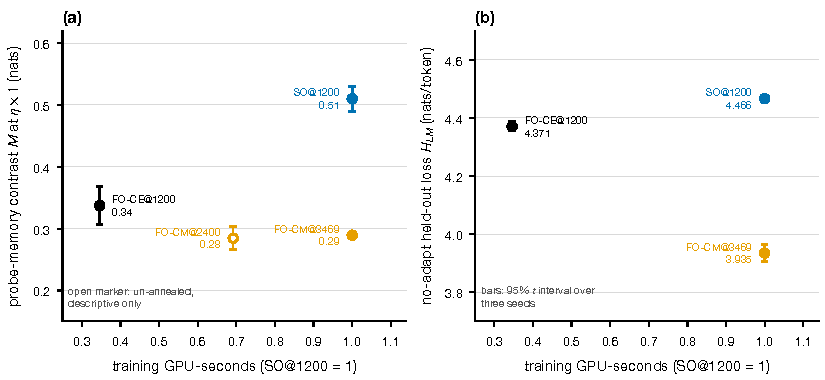
\includegraphics[width=\linewidth]{figs/figc1-trajectory.pdf}
  \caption{\textbf{\FO-CM's extra GPU-seconds lowered the no-adapt loss, while its default-$\eta$
  probe memory stayed well below \SO's (original study, three seeds; descriptive).} (a) $M$ at
  $\eta\times1$; (b) no-adapt held-out loss $H_{\text{LM}}$, both against the training GPU-seconds.
  Filled markers are annealed endpoints; the open marker is the un-annealed \FO-CM@2400 checkpoint
  (descriptive only); no line joins the checkpoints. $r=2.891$ puts \FO-CE@1200 at 0.35, \FO-CM@2400
  at 0.69 and \FO-CM@3469 at 1.0. Bars, two-sided 95\% $t$-intervals over the three seeds.}
  \label{fig:c1}
\end{figure}

\begin{figure}[!htbp]
  \centering
  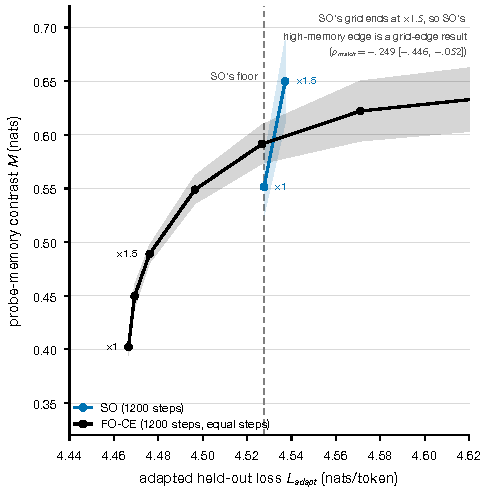
\includegraphics[width=3.25in]{figs/figc2-minis-frontier.pdf}
  \caption{\textbf{At mini-s, at matched loss \FO-CE{} matches or exceeds \SO's probe memory (three
  seeds; equal tokens).} $\rho_{\text{match}}=-.249$ [$-.446$, $-.052$]. \SO's $\eta$ grid ends at
  $\times1.5$, so \SO's high-memory edge there is a grid-edge result. Lines join the seed means at each
  measured $\eta$; bands are two-sided 95\% $t$-intervals of $M$ over the three seeds. The $x$-axis
  $L_{\text{adapt}}$ is the adapted loss on all 128 held-out documents (Fig.~\ref{fig:frontier} uses
  their \textsc{cal} half).}
  \label{fig:c2}
\end{figure}

\FloatBarrier

\section{The released TTT-E2E continuation}
\label{app:125m}

We continued the released TTT-E2E 125M checkpoint \citep{tandon2025e2e} (DCLM, 8K context, step 4799)
for 400 outer steps of $64\times8192$ tokens (about 210M tokens) under \SO{} and \FO-CE, one run per
arm, from the same weights and data order. The released peak learning rate $3\times10^{-3}$
destabilised \SO{} during re-warm-up (a registered pilot check aborted it at step 30), so both arms
used a peak of $10^{-3}$. Unlike the toy, the inner clip scale is not detached, so \SO{} also
differentiates through it. \FO{} opens a small, stable memory deficit, about a third of the registered
minimum effect, with no \FO{} language-model advantage. The copy signature the toy predicts does not
appear: sources that attention could copy had a write-time inner error about 39\% smaller, but equally
in both arms. The caveats: one run per arm, a peak learning rate of $10^{-3}$,
domain-cluster intervals that do not cover training-seed variance, and the comparison is neither
compute-matched nor a confirmation of the equal-GPU-second result.

\begin{table}[!htbp]
\centering
\caption{125M continuation, endpoint at step 400. $D=L_{\FO}-L_{\SO}$ on barrier probes;
$\Delta M=M_{\SO}-M_{\FO}$, the original endpoint estimate; copy contrast
$K=D_{\text{copyable}}-D_{\text{barrier}}$. The write/read split comes from a separate writer--reader
swap re-evaluation, whose total is $.0147$ (see text). Intervals are 90\% URL-domain cluster
bootstraps over documents; with one run per arm they do not cover training-seed variance.}
\label{tab:125m}
\small
\begin{tabular}{@{}lcc@{}}
\toprule
Measure & Value & Interval \\
\midrule
$D$ (probe loss gap, FO minus SO) & $+.0180$ & $[+.0163,+.0197]$ \\
$\Delta M$ (focal memory, original endpoint) & $+.0143$ & $[+.0134,+.0151]$ \\
held-out LM gap (no FO advantage) & $+.0007$ & --- \\
copy contrast $K$ (registered) & $+.0069$ & $[-.0109,+.0241]$ \\
\quad sensitivity (both sources in segment 2) & $+.0186$ & $[+.0011,+.0367]$ (nominal) \\
\quad predictable-at-write stratum & $-.0142$ & $[-.0173,-.0110]$ \\
write-time inner error, \FO/\SO{} ratio & .995--1.000 & --- \\
swap re-evaluation: write / read & .0070 / .0077 & [+.0064, +.0075] / [+.0072, +.0082] \\
write cosine, FO vs SO & .97--.99 & --- \\
focal write size (FO vs SO) & 3--8\% smaller & --- \\
\bottomrule
\end{tabular}
\end{table}

\paragraph{Probes and focal memory.} Each 8192-token document is split into two source segments and
a probe segment, with the attention context reset at each boundary; a probe is the last token of the
first occurrence in the probe segment of a 4-gram that also occurs in a source segment. Focal memory
$M$ is the probe loss with the source tokens' inner-loss terms removed, minus the loss with the same
number of other source-segment tokens removed in each chunk; the probe segment does not write while
$M$ is measured.

\paragraph{Write/read swap.} A writer reads the source segments; its fast-weight change from its own
$W_0$ is added to the reader's $W_0$; the reader then reads the probe with its own slow weights,
without writing. Let $Q_{ry}$ be the focal memory with reader $r$ (which also supplies its $W_0$)
and writer $y$, each \SO{} ($s$) or \FO-CE{} ($f$). Writing gets
$\tfrac12[(Q_{ss}-Q_{sf})+(Q_{fs}-Q_{ff})]$ and reading $\tfrac12[(Q_{ss}-Q_{fs})+(Q_{sf}-Q_{ff})]$,
summing to the swap's own $\Delta M=Q_{ss}-Q_{ff}$. On a single GPU this re-evaluation gives a total
of $.0147$ (write $.0070$, read $.0077$), against the original endpoint estimate $.0143$ from the
training GPUs; the $+.00046$ difference is a cross-device re-evaluation difference, within the
registered validation tolerance ($1.1\times10^{-3}$). The allocation is
convention-dependent: if the writer starts from the reader's $W_0$, writing gets about 27\% and reading
73\%.

\FloatBarrier

\section{Two other domains: SCM and WM2}
\label{app:domains}

Both studies are separate projects with their own registrations; neither is compute-matched, and
neither is pooled with the echo counts. They bear on the write target, not on the text budget
question; keep-versus-revise was not measured on text.

\paragraph{SCM.} SCM trains the toy model of \S\ref{sec:toy} on a symbolic world stream whose stored
locations change by an agent action that copies its argument (A) or sets a uniform value (Au), and by a
first binding at a never-observed location (N). At $\eta=10$, no fixed \FO{} write rule tried in the
first remedy phase keeps A, Au and N together, while \SO-CE{} keeps every scored change type in 6/6
seeds (registered; two rule-based types are descriptive only; at $\eta=40$ the \SO{} reference was not
competent). A first-order linear write applied only at the action tokens, with a per-token weight tied
to the token's read-out scale $\sigma_t$ (capped at 4), was chosen after that phase and then kept A, Au
and N in 6/6 fresh seeds (a post-result gate). SCM's registered agency contrast, agent against
exogenous changes of matched predictability, was null: in that toy, loss follows predictability at the
write, not who caused the change (we read). A residual floor applied at every position from the start
of training did not keep first bindings (N, 0 of 6); that is a different task, layout and start, so it
is not a site control for \S\ref{sec:chron}.

\paragraph{WM2: task and arms.} WM2 is a visual hidden-object task: a ball is shown, covered by a cup,
and then either left in place (\emph{keep}, N) or secretly moved and revealed when a cup is lifted
(\emph{revise}, X). Memory is read beyond a 7-frame attention window, at delays $L=12/24/48$ frames.
Three TTT arms share a fixed step size and write after every frame: E2E-\FO, whose inner loss is the
whole model's next-frame MSE (WM2's end-to-end target; not the CE of the toy and text), with the write
gradient detached; an \FO{} arm whose inner loss scores only the memory's own contribution (AICE-\FO);
and E2E-\SO, with the same MSE inner loss at second order. The registered claims
were: E2E-\FO{} fails to keep but revises; AICE-\FO{} keeps but does not revise; E2E-\SO{} keeps
($E_N\ge.90$) and revises only partly ($R_X<.85$).

\begin{table}[!htbp]
\centering
\caption{\textbf{WM2, registered read on fresh evaluation episodes (original three training seeds).}
Every column is an AUROC over the three cup places (chance .5); subscript N: keep episodes, X: revise
episodes. The read score $\alpha_q$ projects the predicted frame onto the difference between the twin
frames with and without the ball under place $q$. $R$: AUROC of $\alpha$ (the behavioural read); $E$:
AUROC of the memory-effect score $\alpha-\alpha(W_0)$, the read minus the same read with the fast
weights reset to $W_0$; X\_old: AUROC of the read toward the old location after revision. Thresholds
fixed before the data. The read on five fresh training seeds (101--105) confirmed the three
claims 5/5, 5/5 and 4/5 against a registered $\ge4/5$ rule; the \SO{} exception (seed 101,
$R_X=.863$) revised more than the ceiling allows.}
\label{tab:wm2}
\small
\setlength{\tabcolsep}{3pt}
\begin{tabular}{@{}llcccccc@{}}
\toprule
& & & \multicolumn{5}{c}{AUROC} \\
\cmidrule(l){4-8}
Claim & Arm & Seeds & $R_N$ & $R_X$ & $E_N$ & $E_X$ & X\_old \\
\midrule
fails to keep, revises & E2E-\FO{} & 3/3 & .50--.56 & .87--.92 & .54--.60 & .93--.95 & .31--.34 \\
keeps, does not revise & AICE-\FO{} & 3/3 & .87--.96 & .33--.47 & .88--.97 & .36--.49 & .81--.95 \\
keeps, revises partly & E2E-\SO{} & 2/3 & .99--1.00 & .73/.87/.75 & 1.00 & .74--.86 & .63--.77 \\
\bottomrule
\end{tabular}
\end{table}

\paragraph{WM2: caveats.} (i) \SO{} costs 2.3--2.9$\times$ \FO{} per step and was not compute-matched.
(ii) On the training runs' own evaluation episodes (not the fresh episodes of Table~\ref{tab:wm2}), a
GRU reaches $N=.999$ and $X=.821$, against $X=.767$ for \SO{}, at a step 12.6$\times$ cheaper than \SO's;
at 400 dark frames \SO{} keeps the shown location (1.00 against .59), while the GRU revises better
(.90 against .77; the paired difference $-.14$ [$-.24$, $+.03$], a 95\% bootstrap over seeds and episodes, includes
zero). All descriptive. (iii) The
fresh-seed claim on \SO{} is partial revision (4/5), and the failing seed failed by revising more.
(iv) The mechanism analyses (an intervention on the read and the size of the location signal in the
writes) are post hoc; the absence of erasure is not proven; the five fresh seeds share one training
corpus. (v) Discriminability of the stored location is not calibrated belief. (vi) A higher-step-size
\SO{} arm diverged in all three seeds. (vii) No fixed or switched mix of the two \FO{} targets passed
keep, revise and the control in two seeds; such mixes trade keeping for revising along one curve.
(viii) Keep-versus-revise was not measured on text. We read WM2's mechanism as only partly the
toy's. E2E-\FO's total show write is not starved: $\gamma_{\text{show}}$, the registered ratio of the
median update norm of writes targeting the show and cover frames to the median, over episodes, of
the largest write between the command and the lift, is .74--.86 over both step sizes. Post hoc, a
read-time analysis of the lower-step-size checkpoints finds a weaker location-related signal: the place-mean signal in E2E-\FO's show writes is .10--.46 of that in
its lift writes, although the location stays decodable from the memory's response (probe .71--.85,
chance .33). This is consistent with content-selective suppression of a write that is predictable
where it is made, and does not identify a cause during training.

\FloatBarrier

\section{Hyperparameters and timing}
\label{app:hparams}

\begin{table}[!htbp]
\centering
\caption{Text-model settings, read from each run's configuration. mini-m is every text claim unless
stated; mini-s (5.12M non-embedding, 0.88M fast, 37.95M total) appears once in
Appendix~\ref{app:protocol}; 125M (85.86M non-embedding, 184.36M total) in \S\ref{sec:mechanism} and
Appendix~\ref{app:125m}. Counts from \texttt{param\_count()}.}
\label{tab:hparams}
\scriptsize
\begin{tabular}{@{}L{2.6cm}L{10.9cm}@{}}
\toprule
Setting & Value \\
\midrule
\textbf{All text} & \\
Model (mini-m) & 25.6M non-embedding parameters (91.3M total; the tied $128{,}256\times512$ embedding is
65.67M), 3.44M fast weights in the last two blocks. \\
Layout & $T=8192$, chunk 1024; attention and RoPE reset at chunks 2, 4, 6 ($S=2048$); global batch 16
sequences ($131{,}072$ tokens/step). \\
Inner loop & CE next-token loss; per-sequence fast weights from $W_0$; inner step size multiplied by
$\eta$ at eval time; no retraining per frontier point. \\
Train data & DCLM rows, sequential; \FO-CM's steps 1--1200 reuse \FO-CE's rows, only
3201--$N_{\text{CM}}$ touch the third split. \\
\textsc{cal}/\textsc{test} & Even/odd indices of 128 adapted-loss documents; $\eta$ chosen on \textsc{cal};
$M$ on 1024 separate documents. \\
\midrule
\textbf{Arms} & \\
\SO, \FO-CE & 1200 steps; micro-batch 1 (\SO) and 2 (\FO-CE). \\
\FO-CM{} & 3469 steps, micro-batch 4; \FO-CE's recipe with the horizon and both warm-ups (outer and
inner, 347 steps) stretched; cosine; nothing else re-tuned. \\
\FO-WSD{} & 1200 or 3469 steps, micro-batch 4; outer learning rate warm-up over 120 steps to
$3\times10^{-3}$, constant, then linear decay to $10^{-5}$ over the last 240 steps; inner warm-up
.1$\to$1 over 120 steps, then constant, as \FO-CE. \\
\SOp{} & \SO{} on 2 of 16 rows per batch, \FO{} on the rest; $N_P=2793$ fixed from the pilot before
training; warm-up $\mathrm{round}(.1N_P)$, cosine; \SO{} rows at micro-batch 2. \\
\midrule
\textbf{Compute match (RTX 4090)} & \\
Timing pilot & \SO{} fastest at micro-batch 2 (6607\,ms, 14.9\,GB), \FO{} at 4 (2285\,ms, 18.8\,GB);
$r=2.891$; counted FLOP ratio 2.02; $N_{\text{CM}}=1200r=3469$. Replication pilot: $r=2.901$,
$\rho=.997$. \\
Realised & Original: $r_{\text{act}}/r=1.0017/1.0034/1.0015$ (raw .997/.992/.997). Replication:
$r_{\text{act}}/r$ .985--1.024. Against \SO's realised micro-batch-1 training, $\rho\approx.92$. \\
Tokens & 157M (1200 steps), 455M (3469 steps). \\
125M profile & 79.4\,s (\SO) against 21.6\,s (\FO) per outer step of $64\times8192$ tokens, one RTX 5090
($3.7\times$). \\
\bottomrule
\end{tabular}
\end{table}

\begin{table}[!htbp]
\centering
\caption{Toy hyperparameters and run recipe, shared by the echo, copy-free, Markov and load runs;
run-level departures are in the last row. $s$ is the run seed.}
\label{tab:toy-hparams}
\scriptsize
\begin{tabular}{@{}L{2.7cm}L{10.7cm}@{}}
\toprule
Setting & Value \\
\midrule
Echo task & $T=512$, $V=50$ (write and query markers, 16 keys, 16 values and 16 fillers); 16 write events
in chunk 0, then a 268-token filler and one query per key, at positions 333--430 in the evaluation set.
Each sequence draws its own map from 16 keys to 16 values, uniformly with replacement. \\
Backbone & Four pre-LN transformer blocks, $d=128$, four heads, RoPE base $10^4$, GELU MLP width 512,
causal sliding-window attention of width $w=64$ and receptive field 253; learned token embedding,
final LayerNorm and untied unembedding without bias. \\
Fast head & $h+W_2\,\mathrm{gelu}(W_1x+b_1)+b_2$, hidden width 512; $x=\mathrm{LN}(h)$, or
$(\mathrm{LN}(h)+\tilde E[\mathrm{tok}])/\sqrt2$ in $+$emb arms. $\tilde E$ has Gaussian rows scaled to
unit RMS, with generator seed $s+7919$, and is not trained. \\
Initialisation & Weights $\mathcal N(0,0.02^2)$, biases zero, attention and MLP output projections
scaled by $1/\sqrt8$, $\rho=0$, PyTorch seed $s$. Parameter counts are 938{,}116 (echo, $V=50$),
933{,}508 (Markov, $V=32$), and 999{,}556 (load, $V=290$), plus one parameter for a separate kv step
size. \\
Inner loop & Per-sequence fast weights $(W_1,b_1,W_2,b_2)$ start from learned $W_0$; $C=T/64$ chunks;
mean next-token CE unless the arm changes it; joint gradient norm clipped to 10 per sequence with
detached scale. $\eta_i=\eta_{\text{base}}\exp(\rho_i)$, one per fast tensor; learned $\rho$ uses
learning rate $10^{-2}$ and fixed runs use $\eta=\eta_{\text{base}}$. \\
Outer loop & AdamW with $\beta=(0.9,0.95)$, peak learning rate $10^{-3}$, weight decay 0.01 on
matrices, gradient-norm clip 1, batch 32; 200 warm-up steps, then cosine decay from peak at step 200
to $0.1$ times peak at the schedule length, which is 3000 for the echo, copy-free and load runs (the
Markov exception is in the next row); echo runs stop at step 1500, where the last update uses $0.60$
times peak. \SO{} uses \texttt{create\_graph=True}; \FO{} treats each inner gradient as
constant. \\
Run recipe & Main echo arms use learned $\eta$ at base 10, fixed-$\eta$ arms use $\eta\in\{10,40,160\}$,
and the fresh fixed-$\eta$ replication uses $\eta=40$; copy-noise arms use $q\in\{1,3,5,10\}\%$ and
filler controls match the expected 5\% count; load runs use $N\in\{16,32,64,128\}$ pairs at fixed
$\eta=10$ for 1500 steps; the Markov task uses $T=1024$, $V=32$, Dirichlet$(0.1)$ rows, learned $\eta$
at base 0.3 and 4000 steps, schedule length 4000. \\
Evaluation & Full echo evaluation uses 256 sequences and 4096 queries; quick evaluation uses 64
sequences; probe evaluation uses 32 sequences and 512 kv events. Training streams are shared across
paired arms; copy-noise draws use a separate stream. \\
Run-level departures & First comparison: 3000 steps. Random-prefix layout: $T=640$, prefix 64--192,
2000 steps (schedule length 4000) at peak $5\times10^{-4}$. Step-size sweep: $\eta_{\text{base}}\in\{3,30\}$,
learned, \FO{} only. Linear-loss experiment: one arm with 600 warm-up steps. Load budget extension: 3000 steps, to the end of
the schedule. \\
\bottomrule
\end{tabular}
\end{table}

\FloatBarrier

\section{Experiment index}
\label{app:index}

Every experiment series of the project, including negative results, with what it was, its outcome,
the claim it bears on and the repository folder holding its result files; engineering-only runs
(pipeline tests, timing profiles) are omitted. ``Original study'' is SOQ-N3B; ``the replication'' is S14-R. S: supported, F: falsified, I: inconclusive, NE: not evaluable.

\scriptsize
\setlength{\tabcolsep}{2.5pt}
\def\UrlBreaks{\do\/\do\-\do\_\do\.}
\begin{longtable}{@{}L{1.9cm}L{3.2cm}L{3.5cm}L{1.6cm}L{2.8cm}@{}}
\toprule
Series & What it was & Outcome & Bears on & Result files \\
\midrule
\endfirsthead
\toprule
Series & What it was & Outcome & Bears on & Result files \\
\midrule
\endhead
\bottomrule
\endfoot
\multicolumn{5}{@{}l}{\emph{Text: the budget test and its replication}} \\
SOQ-N3B (+pilot, 3 FO-CM seeds, 4 read jobs) & original study: FO-CM at equal GPU-seconds, frontier reads, $\kappa$ & not covered (large); $x$ no closer; damage flag on all seeds & \S\ref{sec:gpu}, Table~\ref{tab:main} & \nolinkurl{results/text-original-study/} \\
A0 cross-fit audit & cross-fit selection on the original study's reads (no training) & labels unchanged; seed 2 FO-CM moves in one fold & \S\ref{sec:setup}, App.~\ref{app:protocol} & \nolinkurl{results/text-crossfit-audit/} \\
S14-R (12 GPU jobs) & replication: 6 arms $\times$ seeds 3--5, training, reads, passkey & FO-CM replicates (.139); $x$ below FO-CE, narrow (\S\ref{sec:steps}); WSD not covered; SO-2/16 underpowered; passkey interval & \S\ref{sec:text}, \S\ref{sec:mechanism} & \nolinkurl{results/text-replication/} \\
Equal-token check & post hoc re-reading of the original study at equal tokens & two-sided frontier; $\eta$-inflation controls & \S\ref{sec:price} & \nolinkurl{results/text-equal-token-check/} \\
XPO-0 & exposure of cross-segment repeats, DCLM vs code & 1.61\% of DCLM targets & \S\ref{sec:price} & \nolinkurl{results/text-repeat-exposure/} \\
\midrule
\multicolumn{5}{@{}l}{\emph{Text: mechanism diagnostics and levers (mini-m, mini-s)}} \\
MINI & from-scratch mini-m/mini-s: SO, FO-CE, residual-floor arms & equal-step gap $\Delta M(1)=.173$; floors $\le3\%$ & \S\ref{sec:recover}, Table~\ref{tab:knobs} & \nolinkurl{results/text-mini-baseline/} \\
MINI-D & copyable vs distance split of the deficit & distance-like & \S\ref{sec:mechanism} & \nolinkurl{results/text-copyability-distance/} \\
MINI-A & write--read alignment & alignment hypothesis not supported & \S\ref{sec:mechanism} & \nolinkurl{results/text-write-read-alignment/} \\
MINI-E & eval-carried read of the residual floors & $\bar C_E\approx0$; starvation class NE; cotangent .935 (F) & Table~\ref{tab:knobs} & \nolinkurl{results/text-floors-eval-read/} \\
MINI-P & partial SO (2/16 rows) at equal steps & $\phi=.20$; no transfer at equal steps & Table~\ref{tab:knobs} & \nolinkurl{results/text-partial-so-equal-steps/} \\
MINI-L & 300 late SO steps after FO-CE & late-fails ($\psi=.196$) & Table~\ref{tab:knobs} & \nolinkurl{results/text-late-so/} \\
TBB & reduced-vocabulary micro testbed & not qualified (relative gap only) & background & \nolinkurl{results/text-micro-testbed/} \\
G0 & write-gain split; eval-time $\eta$ and $\sigma$-CE & partial dose; $\sigma$-CE adverse & \S\ref{sec:mechanism}, Table~\ref{tab:knobs} & \nolinkurl{results/text-write-gain/} \\
G0b & matched-loss frontier; inverse-$\sigma$ rule & frontier match at SO's default $\eta$ only; inverse $\sigma$ .176 & \S\ref{sec:price}, Table~\ref{tab:knobs} & \nolinkurl{results/text-matched-loss-frontier/} \\
G0c & inverse-$\sigma$ $\times$ $\eta$ frontier lift & unresolved (.071) & Table~\ref{tab:knobs} & \nolinkurl{results/text-inverse-sigma-lift/} \\
SOQ-FS & mini-s matched-loss frontier & $\rho_{\text{match}}=-.249$; gap trends up with size & App.~\ref{app:protocol} & \nolinkurl{results/text-mini-s-frontier/} \\
SOQ-V1 & echo-in-text template validity & registered fail, instrument-caused & \S\ref{sec:mechanism} & \nolinkurl{results/text-echo-template/} \\
SOQ-P1-0, -0c & injected-binding pilot & fail through a design shortcut (key-agnostic priming) & App.~\ref{app:protocol} & \nolinkurl{results/text-injected-binding-pilot/} \\
SOQ-P1-v3, -v3x, -v3p & injected binding v3; late-storage check; post hoc reads & not learnable; no late storage & \S\ref{sec:mechanism} & \nolinkurl{results/text-injected-binding/} \\
\midrule
\multicolumn{5}{@{}l}{\emph{Released 125M model}} \\
P2-0 & port and timing profile of the released 125M & SO/FO step time 3.7$\times$ & App.~\ref{app:hparams} & \nolinkurl{results/125m-timing/} \\
P2-1 & 400-step continuation, SO vs FO-CE & small FO deficit ($D=+.0180$); copy contrast not passed & \S\ref{sec:mechanism}, App.~\ref{app:125m} & \nolinkurl{results/125m-continuation/} \\
P2-2 & write/read swap & split .0070 / .0077 & App.~\ref{app:125m} & \nolinkurl{results/125m-write-read-swap/} \\
\midrule
\multicolumn{5}{@{}l}{\emph{Toy: the phenomenon and its barriers}} \\
R1 & first FO vs SO comparison (1--2 seeds) & FO does not bind on echo; on the Markov task FO keeps 96\% of SO's gain & \S\ref{sec:twobarriers} & \nolinkurl{results/toy-first-comparison/} \\
R2 bundle & random-prefix layout, Jacobian-SO, copy-free control & anchor gate fired; SO bistable & background & \nolinkurl{results/toy-layout-bundle/} \\
R2b & six-seed contrast & SO binds 4/6, FO 0/6 & \S\ref{sec:twobarriers} & \nolinkurl{results/toy-six-seed-contrast/} \\
R3 & random-prefix binding; $\eta$ sweep & I: no random-prefix arm binds (0/6 each); $\eta$ sweep 0/3 each & App.~\ref{app:toy} & \nolinkurl{results/toy-random-prefix/} \\
R2-4 & write-position ablation (eval only) & kv write necessary and sufficient, 7/7 & \S\ref{sec:starved} & \nolinkurl{results/toy-write-ablation/} \\
R2-4b & key addressability probes & FO: content-failure criterion 4/6, address criterion 0/6 (mixed) & \S\ref{sec:twobarriers} & \nolinkurl{results/toy-key-address/} \\
R4-0 & write-code rank diagnostics & codes collapsed; marker supplies the answer & background & \nolinkurl{results/toy-write-code-rank/} \\
R4-1 & key/error/embedding arms $\times10$ & SO 7/10 acq., 6/10 ret.; FO$+$emb 10/10 acq., 0/10 ret. & Table~\ref{tab:twobarriers} & \nolinkurl{results/toy-key-code-arms/} \\
TH-RC & fixed-$\eta$ retention & FO-CE 0/18 vs SO 15/18 & Table~\ref{tab:twobarriers} & \nolinkurl{results/toy-fixed-eta-retention/} \\
FRS-A & fresh-seed pool (FO 200--215, SO/noise 200--211) & headline replicated & \S\ref{sec:twobarriers} & \nolinkurl{results/toy-fresh-seed-replication/} \\
\midrule
\multicolumn{5}{@{}l}{\emph{Toy: chronology and interventions}} \\
R4-2 & outer-loss mask at kv & 10/10 vs 0/10; mediator 6/10 (req. 8/10) & Table~\ref{tab:interventions} & \nolinkurl{results/toy-outer-mask/} \\
R4-2L & linear inner loss, schedule and copy-free controls & 10/10 at kv and everywhere; site control 0/10 & Table~\ref{tab:interventions}, \S\ref{sec:toyfix} & \nolinkurl{results/toy-linear-inner-loss/} \\
R4-3 & second-order halves; mask replication & 10/10 and 9/10; mask 10/10 vs 0/10 & App.~\ref{app:toy} & \nolinkurl{results/toy-so-halves/} \\
R4-4a & copy-edge mask, copy noise, Kamin two-stage \citep{kamin1969predictability}, kv step size & rows of Table~\ref{tab:interventions} & Table~\ref{tab:interventions} & \nolinkurl{results/toy-copy-interventions/} \\
R4-4b & AICE rule, Kamin repeat \citep{kamin1969predictability} & AICE equals linear in chunk 0; joint criterion not met & App.~\ref{app:theory} & \nolinkurl{results/toy-aice-kamin/} \\
R4-4c & toy rehearsal of the 125M continuation & re-warmed SO 10/10 vs FO-CE 0/10; linear 10/10 & App.~\ref{app:125m} & \nolinkurl{results/toy-125m-rehearsal/} \\
BW1a, BW1b & fixed-$\eta$ copy noise & threshold in $(1\%,3\%]$ & App.~\ref{app:toy} & \nolinkurl{results/toy-noise-floor/} \\
CHR & dense chronology and acquisition forks & starvation-starts prediction F (0/6) & \S\ref{sec:chron}, Fig.~\ref{fig:chr} & \nolinkurl{results/toy-chronology/} \\
TRG & trigger of the loss & trigger not identified; outer mask prevents 14/15 & \S\ref{sec:chron} & \nolinkurl{results/toy-trigger/} \\
RDO-RPE & recovery dose and prevention floors & floor .03: 12/12 vs 1/12; prevention not kv-specific & \S\ref{sec:chron}, App.~\ref{app:toy} & \nolinkurl{results/toy-recovery-prevention/} \\
POOL & combined fresh-seed runs (40 main runs, 316 forks) & runs for FRS-A, TRG, RDO-RPE & \S\ref{sec:chron} & \nolinkurl{results/toy-fresh-seed-pool/} \\
\midrule
\multicolumn{5}{@{}l}{\emph{Toy: the write target and its price}} \\
P0.0 & Markov-task cost of the linear loss & linear beats FO-CE by .026 & \S\ref{sec:toyfix} & \nolinkurl{results/toy-markov-cost/} \\
P0.1 & mechanism probes (logit split, copy edge, re-assignment) & gate pass 9/9; linear keeps old map & \S\ref{sec:toyfix} & \nolinkurl{results/toy-mechanism-probes/} \\
SOQ-D (P3-a) & write-rule control & DiD $+.454$; own-residual fails control 4/6 & \S\ref{sec:toyfix} & \nolinkurl{results/toy-write-rule-control/} \\
FRS-B & plain echo $\times$ \{CE, linear\} & linear without code 0/12 & \S\ref{sec:toyfix} & \nolinkurl{results/toy-plain-echo-linear/} \\
B9 & address auxiliary & 12/12 vs 0/12 filler & \S\ref{sec:toyfix} & \nolinkurl{results/toy-address-auxiliary/} \\
LOD & load scaling, $N=16$--128 & linear behind SO at 32 & App.~\ref{app:toy} & \nolinkurl{results/toy-load-scaling/} \\
LOD-X & budget extension to 3000 steps & 32-pair price not reproduced (fragile) & App.~\ref{app:toy} & \nolinkurl{results/toy-load-extension/} \\
RTW & per-token write-gain gate; partial-SO screen & gate closed (0/12); $p=1/8$ 11/12, late 12/12, early 1/12 & App.~\ref{app:toy} & \nolinkurl{results/toy-partial-so-screen/} \\
RTW-C & registered partial-SO confirmation & $p=1/8$ 12/12; late 12/12 & App.~\ref{app:toy} & \nolinkurl{results/toy-partial-so/} \\
\midrule
\multicolumn{5}{@{}l}{\emph{Other domains and theory}} \\
E1-VE, -D, -D2, -D3, -D4 & world-model echo; diagnostics & predecessor of SCM & App.~\ref{app:domains} & \nolinkurl{results/visual-echo/} \\
SCM & symbolic world stream, separate project & SO keeps A/Au/N 6/6; action-selective FO linear write 6/6 (post-result) & \S\ref{sec:toyfix}, App.~\ref{app:domains} & \nolinkurl{results/scm/} \\
WM2 & visual hidden object, separate project & keep/revise pattern confirmed (5/5, 5/5, 4/5) & \S\ref{sec:toyfix}, App.~\ref{app:domains} & \nolinkurl{results/wm2/} \\
Theory loops A, B & performative correspondence; key--pair model; reduced model & derived and checked; reduced model's discriminating predictions F & App.~\ref{app:theory} & \nolinkurl{results/theory-checks/} \\
Parameter check & parameter counts of the text models & counts confirmed & \S\ref{sec:setup} & \nolinkurl{results/text-param-counts/} \\
\end{longtable}
\normalsize

\end{document}
